% ========================================================
% Document Class
% ========================================================
\documentclass[journal,article,submit,pdftex,moreauthors]{Definitions/mdpi} 
\makeatletter
\let\@citation\relax
\let\@journalname\relax
\let\@articlenumber\relax
\let\@journalvolume\relax
\let\@journalyear\relax
\let\@journalpages\relax
\makeatother
% ========================================================
% Page & Document Metadata
% ========================================================
\firstpage{1} 
\makeatletter 
\setcounter{page}{\@firstpage} 
% \includegraphics[width=0.1\textwidth]{denison.png}
% Remove journal header metadata
\def\@journalname{}
\def\@articlenumber{}
\def\@journalvolume{}
\def\@journalyear{}
\def\@journalpages{}

% Suppress submission/publication metadata
\renewcommand{\datereceived}{} 
\renewcommand{\dateaccepted}{} 
\renewcommand{\daterevised}{} 
\renewcommand{\datepublished}{} 

\makeatletter
\def\@journalDates{}
\makeatother

% ========================================================
% Package Imports
% ========================================================
\usepackage{natbib}
\setcitestyle{authoryear,open={(},close={)}}
\bibliographystyle{apalike}

\usepackage{titlesec}
\usepackage{pdflscape}
\usepackage{fancyhdr}
\usepackage{lastpage}
\usepackage{color}
\usepackage{graphicx}
\usepackage{float}
\usepackage{caption}
\usepackage{xcolor}
\usepackage{comment}

% ========================================================
% Fancy Header Setup
% ========================================================
\pagestyle{fancy}
\fancyhf{} % clear all header and footer fields

\fancyhead[L]{\footnotesize Version April 30, 2025}
\fancyhead[R]{\footnotesize Page \thepage\ of \pageref*{LastPage}} % No hyperlink

\renewcommand{\headrulewidth}{0.4pt} % top line thickness
\renewcommand{\footrulewidth}{0pt}   % no bottom line

% Redefine the actual headrule so the black line appears
\makeatletter
\renewcommand{\headrule}{\hbox to\headwidth{%
  \color{black}\leaders\hrule height \headrulewidth\hfill}}
\makeatother

% Remove header from title (first) page
\fancypagestyle{plain}{
  \fancyhf{}
  \renewcommand{\headrulewidth}{0pt}
  \renewcommand{\footrulewidth}{0pt}
}

% Full title of the paper (Capitalized)
\Title{Population Density and Housing Price Dynamics:\\A Comparative Analysis of the Southeastern and Midwestern United States}

% MDPI internal command: Title for citation in the left column
\TitleCitation{Denison University}

% Author Orchid ID: enter ID or remove command
%\newcommand{\orcidauthorA}{0000-0000-0000-000X} % Add \orcidA{} behind the author's name
%\newcommand{\orcidauthorB}{0000-0000-0000-000X} % Add \orcidB{} behind the author's name

% Authors, for the paper (add full first names)
\Author{M. Christian McIntire$^{1*}${}}

%\longauthorlist{yes}

% MDPI internal command: Authors, for metadata in PDF
\AuthorNames{Christian McIntire, Alexandre Scarcioffolo}


% Affiliations / Addresses
\address{%
$^{1}$ \quad Department of Data Analytics, Denison University; \texttt{ mcinti\_c1@denison.edu}, \texttt{christianmcint@gmail.com}\\
}

% Contact information of the corresponding author
\corres{This research was supported by Dr. Alexandre Scarcioffolo, Ph.D., Assistant Professor of Data Analytics}
% \firstnote{Optional note here 1} 
% \secondnote{Optional note here 2}

%\simplesumm{} % Simple summary

%\conference{} % An extended version of a conference paper

% Abstract (Do not insert blank lines, i.e. \\) 
\abstract{
This research studies the relationship between population dynamics and housing price trends in the Southeastern and Midwestern United States, using an observational and comparative data-driven analysis. This paper aims to explore and explain how regional differences between the Southeast and Midwest impact housing affordability and price dynamics, with the Southeast experiencing rapid population growth while the Midwest faces more stagnant population fluctuations. By using publicly available data from the U.S. Census Bureau, Zillow Research, the Federal Reserve Bank of St. Louis, and the National Association of Realtors, a combination of hedonic modeling and ARIMA$^{*}$ time-series analysis is used to explore relationships between population trends and unique housing markets down to a county level. The findings indicate that although population growth is associated with rising housing prices and often mirrors growth trends, mortgage payment levels emerge as a statistically significant predictor of housing prices. State fixed effects were also crucial to understand differences within each region in this study, as states like Virginia and Missouri experience lower home prices than others when population and mortgage payments are controlled for. Conversely, Florida, Tennessee, and North Carolina face higher variability with several outlier counties skewing the results. ARIMA$^{*}$ forecasting models suggest continued upward housing price trends through 2030, with confidence intervals also suggesting the Southeast will experience greater price volatility and more rapid appreciation than that of the Midwest. Through choropleth visualizations and econometric modeling, this research emphasizes the need for regionally tailored housing policies and development strategies. It also focuses on the importance of using comparative regional data when understanding dynamics within the United States housing market. This research concludes with implications for planners, policymakers, and investors seeking to navigate affordability and growth in the Midwestern and Southeastern United States.
}

% Keywords
\keyword{ARIMA: AutoRegressive Integrated Moving Average} 


%%%%%%%%%%%%%%%%%%%%%%%%%%%%%%%%%%%%%%%%%%
\begin{document}
\pagestyle{fancy}
\thispagestyle{empty} % or plain, depending on what you want on page 1
\flushbottom
\raggedbottom

% If using automatic title
%\maketitle

% Or your manual title section here
%%%%%%%%%%%%%%%%%%%%%%%%%%%%%%%%%%%%%%%%%%

\section{Introduction}

\subsection{Research Background}

Housing affordability has become a crucial point of discussion within real estate analytics concerning urban economics and housing policy within recent years. As urbanization in the United States continues to increase, housing affordability remains a significant issue, especially in regions which are experiencing population growth booms \citep{desilver2024}. The Southeastern United States is one such region which has been experiencing these population increases, and the impact of an influx of citizens on housing prices is well documented in high density urban markets. However, regional comparisons have not been as closely researched when analyzing the impact of population density on housing price.

Studies have demonstrated that urban housing markets are influenced heavily by hedonic factors, including proximity to downtown urban centers, infrastructure, and economic growth \citep{sirmans_2005_the}. Despite these hedonic factors, differences in housing demand and land availability also create distinct market patterns across regions. This research will mainly focus on hedonic factors such as population density, but it is important to understand that there are outside factors that do affect housing markets as well. While the Southeastern United States has experienced more rapid population growth and an increase in demand for housing, the Midwestern United States has seen more stable or declining population trends, which has led to differing price dynamics in each region \citep{souders_2016_the}. This research seeks to build on previous research in each of these regions by conducting a comparative analysis between the two regions and identify key drivers of housing price through predictive hedonic modeling to assess future trends. This research also provides a more direct comparison between these two regions by providing in depth visual comparisons through data-driven research and analysis.

\subsection{Research Question and Scholarly Aim}

In this paper, I contribute to the research previously conducted on this topic by providing a direct comparative analysis between the Southeastern United States and the Midwestern United States housing markets. I also delve into the effects and contribution that population growth trends and population density have on these two major regions in the United States. Additionally, the data visualizations allow for a direct analysis, which has not been explicitly completed before in this same manner. My primary research questions are as follows:

\begin{itemize}
    \item How has population density historically affected increases within housing prices in the Southeastern and Midwestern United States?
    \item How can these patterns be measured to predict future changes in the United States housing market?
\end{itemize}

This study contributes to the research on this topic by filling a gap in regional housing price dynamics, by specifying the information and analysis down to a county level. Because the influence of population density is often generalized, a more specific analysis will add insight into this issue through a comparative study. These findings will provide insights for policymakers, real estate analysts, and urban planners in designing housing strategies specific to a region, state, or county discussed in this study.

This research combines several methods within its approach, through a combination of descriptive analysis and hedonic modeling. First, the descriptive analysis consists of a summarization and study of historical trends in housing prices and population density for each region, using data from the United States Census Bureau. Choropleth maps also assist in visualizing spatial distribution by county in each region of the United States. Next, a hedonic model allows for regression models with home price as the dependent variable. Independent variables include population growth, state fixed effects, and mortgage rates. These methods all contribute to understanding how population density does connect with housing prices in both regions, but cannot be studied as the sole predictor factor when studying housing prices in the United States. 

%%%%%%%%%%%%%%%%%%%%%%%%%%%%%%%%%%%%%%%%%%

\section{Literature Review}

The relationship between population density and housing prices is a widely studied phenomenon in urban economics and real estate research. However, existing research studying this topic through a regional lens is scarce, and I aim to add to this field of study by understanding key differences between the Midwestern United States and the Southeastern United States. The Southeastern United States has experienced the most significant population growth, while more Midwestern states have seen more stable or declining population trends, which creates distinct regional variations in housing price dynamics \citep{_2024_net}. This dynamic between different regions of the United States is where many authors have differing views, and I aim to study differences and contribute my own conclusions with the addition of a data analysis driven approach.

This literature review amalgamates existing research pertaining to main factors of housing price, with a focus on population density as a primary driver. In this review, I will briefly explore how hedonic modeling has been used to assess price determinants, discuss methodological approaches in previous studies, and identify any gaps that I believe to be present within this topic. By evaluating these factors and combining prior research from a variety of reputable sources, this literature review will establish a foundation for this research paper to provide a sound analysis between the Southeastern and Midwestern United States within the broader discourse on real estate analytics and economics.

Because housing affordability has become a growing concern in higher density urban markets, especially in rapidly expanding regions, it is important to understand the impacts of population density on housing supply. Rising population levels have strained the housing supply, leading to affordability challenges \citep{desilver2024}. This has been especially noticeable in the Southeastern United States region, leading to my interest in this region within this research. Similarly, increased population density generally raises housing prices, and regional differences such as zoning laws or economic conditions could moderate these increases \citep{a2024_how}.

In addition to affordability, Johnson and Lichter \cite{johnson_2019_rural} highlight rural depopulation trends in the Midwest and explain how regional economic decline could lead to stagnant or declining home prices. This contrasts with the Southeastern increase in population and home prices. These studies focus on the importance of considering regional variations in population growth and housing demand, and the Southeastern and Midwestern regions provide stark contrasts which will be studied in this research.

Hedonic Modeling is widely used to assess various impacts of factors on housing prices. One analysis provides this research with a foundational explanation of hedonic modeling where location, infrastructure, and economic conditions are found to have significant influence on home values \citep{sirmans_2005_the}. Additionally, the Housing Price Index (HPI) is another crucial tool which assists in studying housing prices over time, when adjusted for inflation \citep{suhaida_2011_housing}. While this study does not directly deal with United States housing, it provides a framework for this research to build upon. Additionally, one study by Gupta et al. \cite{gupta_2021_flattening} provides fascinating empirical evidence on how urban housing markets often react to population shifts, notably after the Covid-19 pandemic. These findings indicate that population density might work in conjunction with other external factors to heavily influence housing prices, which is essential to take account of within this research.

Moving on to regional variations, Souders et al. \cite{souders_2016_the} study cross-state variations in population density when looking at effects on housing values. This study shows that factors such as land availability and local economic conditions often counteract price increases in some areas. These are also factors which will be essential to study in this paper as I directly compare states from different regions of the United States. Building on this topic, Holly, Pesaran and Yamagata \citep{holly_2010_a} argue that a spatio-temporal modeling approach can show that regional trends do indeed influence housing markets beyond just a density metric. Combining the methodology and findings from these studies shows that while population growth does affect home price, economic diversification and urban expansion play critical roles as well.  

Many of the studies included within this literature review employ regression-based techniques and hedonic modeling to analyze key determinants within housing price. Suhaida et al. \cite{suhaida_2011_housing} demonstrate that regression modeling can effectively be used when assessing affordability trends , while Holly et al. \cite{holly_2010_a} introduces a spatio-temporal methodology that integrates time series data. Demographic shifts also play key roles within housing price fluctuations, which provides another angle to study within this analysis of regional housing trends \citep{johnson_2019_rural}. However, I believe that despite these studies there is still more information to be desired when analyzing these trends.

\subsection{Literature Review Conclusions}

While many studies within this field analyze housing markets with individual states or regions, very few draw direct comparisons between multiple U.S. regions within this context of population dynamics along with housing prices. This is especially true for both regions focused upon within this study. Additionally, many studies focused on in this literature review offer nationwide trends, which often masks regional or county-level trends. This paper adds to existing literature by providing a direct comparison between the Midwestern and Southeastern regions of the United States. Next, there are limited usages of causal inferences within the studies that have been gathered thus far. Regression models were the dominant methodology, but there are few studies that incorporated advanced econometric methods. Additionally, there are some studies focusing on trends prior to 2020, while this paper emphasizes post-pandemic data to understand how these regions adapted to the pandemic and how it affected the housing markets and population shifts.

This literature review examines existing research on population density and housing prices, and seeks to highlight different findings in affordability, hedonic modeling, regional variations, and methodological approaches. The existing literature surrounding this topic emphasizes the importance of population density as a main determinant of housing prices but also reveals the need for an in-depth comparative analysis which introduces other hedonic factors into the research question. These factors need to be incorporated into the methodology and visualizations of this topic. The findings and inferences from detailed visualizations will allow for policymakers, real estate professionals, and urban planners to understand the evolving relationship between population growth and housing affordability within different regions in the United States.


%%%%%%%%%%%%%%%%%%%%%%%%%%%%%%%%%%%%%%%%%%
\section{Data and Design}

\subsection{Data Documentation}

The data documentation phase of this research is straightforward, and the data presented within this paper is an amalgamation of several comprehensive datasets. Each dataset plays a key role in answering the central research question connecting population density to housing price dynamics in two crucial regions in the United States. The data used comes from four central sources, including the National Association of Realtors \cite{_2024_county}, the Federal Reserve Bank of St. Louis \cite{a2024_hpi}, the United States Census Bureau \cite{_2024_state}, and Zillow Research Data \citep{zillow_2024_housing}. All datasets involved in this research are publicly available and require minimal manipulation and cleaning. The primary methodology consists of hedonic price modeling as well as ARIMA modeling, which connect the necessary variables and allow for predictions of future pricing trends in each region and specific states within each region.

\subsection{Data Collection}

\textbf{National Association of Realtors (NAOR):} The dataset titled \textit{Median Home Prices and Mortgage Payments by County} provides median home prices from the third quarter of 2024 by county \citep{_2024_county}. This dataset is essential for hedonic modeling and for visualizations that demonstrate the drastic variation in county home prices across states and regions. While the raw dataset includes all U.S. counties, this study focuses only on counties within the Southeastern and Midwestern regions. The dataset is cleaned and organized in Excel for better usability within RStudio. It includes county-level median home prices and estimated monthly mortgage payments. The mortgage payment values are not used in this research. The data is converted from PDF to Excel format to enable manipulation and coding.

\textbf{Federal Reserve Bank of St. Louis (FRED):} This source provides state-level housing price index (HPI) data and regional population estimates for the Southeastern and Midwestern United States \citep{a2024_hpi}. The HPI datasets are normalized to a baseline year, making it possible to track changes in housing prices over time. These datasets allow for historical trend analysis and regional comparisons to identify prolonged growth or stagnation across different housing markets.

\textbf{United States Census Bureau (2024):} County-level population estimates and percentage change from 2020–2023 are included for regional comparison \citep{_2023_county}. This data is essential for analyzing population dynamics and for visualizations that correlate population shifts with changes in housing prices.

\textbf{Zillow Research Data (2024):} This exploratory dataset provides the Zillow Home Value Index (ZHVI), which estimates home values using both historical and current market data \citep{zillow_2024_housing}. It includes data for counties, metro areas, and states. The dataset is valuable for time-series modeling and complements the hedonic analysis. The original wide-format CSV is transformed into a long format in RStudio. Missing monthly values are forward-filled to maintain time continuity, and county names are matched to those used in the U.S. Census Bureau and NAOR datasets to ensure consistency across data sources.

\subsection{Data Structure}

The NOAR dataset begins in PDF format and is converted to Excel. It includes columns for state, county, median home price, and mortgage payment. This data is filtered by state and organized by region for hedonic modeling and spatial visualizations \citep{_2024_county}.

The FRED datasets consist of two main types: Housing Price Index (HPI) for each state and population estimates for the Southeastern and Midwestern regions. The HPI datasets allow for time-series analysis of regional home value trends, while the population datasets track demographic changes over time by region \citep{a2024_hpi}. The Census Bureau data includes total population, percentage change, and geographic identifiers for each county from 2020 to 2023. It is used to explore county-level trends in growth and decline, and to relate these changes to housing price fluctuations \citep{_2023_county}. The Zillow Research dataset, while exploratory, contributes valuable insight into housing market dynamics. It contains detailed time-series price information for individual counties, which allows for side-by-side analysis with the NAR median home price data \citep{zillow_2024_housing}. 

Together, these datasets form a foundation for both regression modeling and time-series forecasting, offering a multi-dimensional look at the housing market in these regions of the U.S.

%%%%%% TABLE 1 %%%%%%
\begin{table}[H]
\caption{Data and Design\label{tab:data_design}}
\begin{adjustwidth}{-\extralength}{0cm}
\begin{tabularx}{\fulllength}{>{\raggedright\arraybackslash}p{4cm} >{\raggedright\arraybackslash}p{6.2cm} >{\centering\arraybackslash}p{2cm} >{\centering\arraybackslash}p{2cm} >{\centering\arraybackslash}X}
\toprule
\textbf{Variable Name} & \textbf{Description} & \textbf{Unit} & \textbf{Data Type} & \textbf{Source} \\
\midrule
Median Home Price (Q3 2024) & Median housing price per county in Q3 2024 & USD (\$) & Continuous & NAOR \\
Zillow Home Value Index (ZHVI) & Housing Price Index by county & Index & Continuous & Zillow \\
Housing Price Index (HPI) & Housing Price Index over time & Index & Continuous & FRED \\
State & U.S. state name & N/A & Categorical & Multiple \\
County Name & Name of the County & N/A & Categorical & Multiple \\
Population Estimate (2023) & County-level population in 2023 & Number & Continuous & Census \\
Population Change (2020–2023) & Percentage change in county population & Percentage (\%) & Continuous & Census \\
\bottomrule
\end{tabularx}
\end{adjustwidth}
\end{table}

\subsection{Model Validation}

This paper uses hedonic models to compare Southeast and Midwest housing markets, factoring in population density, region, and other metrics. A well-specified model is critical. \citet{ekeland_2004_identification} note that mis-specified models can produce biased estimates, potentially misleading policymakers or investors. Therefore, careful selection of variables, model structure, and interpretation is vital to support valid and actionable insights.

Spatial visualization techniques that are used within this research, such as choropleth maps, could influence public perception of housing disparities, either by exaggerating or oversimplifying certain areas within the United States. For example, placing an emphasis on counties with the fastest growing home prices, or disproportionately high housing prices may attract high income investors, which can potentially fuel further displacement, and prevent solutions for equitable housing development.

Ethical concerns may also arise when comparing urban housing trends to those of more rural areas, as a direct comparison of the two may not be appropriate in every context within real estate. However, this research provides an exploratory and observational study into the United States housing markets, specifically in the Midwestern and Southeastern regions. These two regions are especially relevant to the overall context of the United States, as the Southeast has experienced severe population growth in comparison to other regions of the United States \citep{biernackalievestro_2023_southern}. In contrast, the Midwestern United States has not experienced such growth, and the comparison of the two has fascinating results \citep{maynard_2021_population}.

%%%%%%%%%%%%%%%%%%%%%%%%%%%%%%%%%%%%%%%%%%
%Ethical Considerations
%%%%%%%%%%%%%%%%%%%%%%%%%%%%%%%%%%%%%%%%%%
\section{Ethical Considerations and Dilemmas}


This project provides several ethical dilemmas and challenges, which are important to address within this paper. While the datasets used for modeling and analysis are publicly available, there may still be several concerns regarding bias, data interpretation, and any potential misuse of the findings. 

One primary ethical concern when considering this research is bias in data representation. This is because housing and demographic data could reflect historical disparities in homeownership, economic development, and urban planning. This research accounts for these potential biases and uses data without any personally identifiable information. Another ethical challenge involves the misuse of the findings resulting from this research. Policymakers, real estate developers, or investors could interpret results in ways that could justify exclusionary zoning laws or other displacement scenarios. Aggregated statistics may unintentionally reveal socioeconomic patterns in vulnerable communities or be misinterpreted in harmful ways. As \citet{brinkmann_2009_putting} argues, real estate data ethics extend beyond legal compliance and require critical evaluation of how data is framed, used, and interpreted. If population density is statistically linked to rising home prices, it could also be considered as justification for pricing out lower-income communities, opposed to addressing growing affordability concerns. Additionally, predictive forecasting with ARIMA models leads to illusions of certainty about future housing trends, which is not the aim of this research, as economic shifts remain unpredictable. This research aims to provide a glance of the current real estate landscape.

\subsection{Context and Relevance}

Spatial visualization techniques used within this research, such as dynamic choropleth maps, could influence public perception of housing disparities, either by exaggerating or oversimplifying certain areas within the United States. For example, placing an emphasis on counties with the fastest growing home prices or disproportionately high housing prices may attract high-income investors, which can potentially fuel further displacement and prevent solutions for equitable housing development. Ethical concerns may also arise when comparing urban housing trends to those of more rural areas, as a direct comparison of the two may not be appropriate in every context within real estate. However, this research provides an exploratory and observational study into the United States housing markets, specifically in the Midwestern and Southeastern regions. These two regions are especially relevant to the overall context of the United States, as the Southeast has experienced severe population growth in comparison to other regions of the United States \citep{biernackalievestro_2023_southern}. In contrast, the Midwestern United States has not experienced such growth, and the comparison of the two has fascinating results \citep{maynard_2021_population}. It is also important to acknowledge that census data may undercount transient or undocumented populations, which could limit the accuracy of conclusions related to population-based dynamics \citep{cooper_2020_on}.

\subsection{Mitigation Strategies}

To address these ethical challenges, this research incorporates several validation techniques and includes transparent findings to prevent any misinterpretation. Bias detection and mitigation strategies are present within the Hedonic Pricing Model through spatial autocorrelation tests. Panel data estimation will include fixed effects modeling within the hedonic model, which will allow for historical and regional controls that may distort results \citep{torresreyna_2010_getting}. 

The ARIMA tests will also include confidence intervals and clear error margins to emphasize forecast uncertainty. The results and visualizations from the ARIMA models do not guarantee future outcomes but instead suggest possibilities for interpreting the publicly provided data. Finally, choropleth maps that are used will include interpretation guidelines, ensuring that color gradients and spatial patterns aren’t misused in any way and instead provide an outline and visual aid to understand patterns within the data.


%%%%%%%%%%%%%%%%%%%%%%%%%%%%%%%%%%%%%%%%%%

\section{Research Design, Methods, and Approach}

This research utilizes a non-experimental and observational research design to analyze the relationship between population density and housing prices in the Southeastern and Midwestern United States. The study explores how historical trends in population growth influence housing price fluctuations by utilizing time series data, and how these patterns can be used for future price prediction. Additionally, given the nature of the publicly available datasets, this study cannot establish strict causal relationships but is able to identify significant statistical associations among present variables through econometric and hedonic modeling.

Because of the observational nature of this study, panel data is also utilized and will account for unobserved, time-invariant factors, reducing omitted variable bias \citep{torresreyna_2010_getting}. Finally, while an experimental study could provide a stronger causal framework, this research with observational methodology is useful for real estate data because of its heavy reliance on past historical market data.

To achieve these results, this study focuses on two primary modeling techniques:
\begin{enumerate}
    \item Predictive modeling using ARIMA – time series forecasting of housing price trends
    \item Hedonic Pricing Model (HPM) – Analyzing housing price determinants and estimating fixed effects by region
    \begin{itemize}
        \item Panel Data Estimation is also utilized within the hedonic model by comparing historical population trends and housing prices across the Southeastern and Midwestern United States.
    \end{itemize}
\end{enumerate}

\subsection{Predictive Modeling: ARIMA (Autoregressive Integrated Moving Average)}

The objective of this methodology is to forecast future changes in housing price indices by using historical pricing data provided by the Federal Reserve Bank of St. Louis. ARIMA modeling is well-suited for time series forecasting, especially for data with high seasonality and historical trends. Further analysis will compare future trends for Southeastern housing price indices with the trends present in the Midwestern housing price data.

The structure of the ARIMA model will consist of Housing Price Index (HPI) per state as the dependent variable. Stationarity and Autocorrelation tests with ACF / PACF tests will be checked to ensure the proper assumptions are met. This model does have several limitations, as ARIMA models rely entirely on historical patterns, and therefore may struggle to predict sudden market shifts. ARIMA models also do not account for any external factors, such as mortgage rates or employment rates \citep{liu_2024_navigating}. The ARIMA model is particularly suited for this study because it captures any temporal trends in the housing price index data, and allows for forecasting of future trends. The dependent variable, Housing Price Index per state, is continuous, while time is an ordered categorical variable.

\subsection{Hedonic Pricing Model (HPM) and Panel Data Estimation}

The objective of the hedonic pricing model within this research is to estimate the impact of location, population density, and economic conditions on housing prices. Hedonic models decompose housing prices into different quantifiable attributes, which makes this method ideal for a comparative analysis of different regions. The structure of the hedonic model will consist of median home price per county as the dependent variable, and will include population, population density, economic indicators, and regional fixed effects as independent variables. The hedonic pricing model is used for cross-sectional analysis, with the dependent variable of median home price per county being continuous, and the independent variables of county and population density being a mix of continuous and categorical variables.

The limitations include potential omitted variable bias, and the assumption that the model assumes a linear relationship. Omitted variable bias could occur if key market drivers are not present within the model, such as interest rates, and the assumption that the model assumes a linear relationship, which has the potential to ignore non-linear dynamics of historical housing prices. Panel data estimation is also included within the hedonic model and includes fixed effects to control for unobserved and time-invariant characteristics \citep{torresreyna_2010_getting}. This methodology will include time series visualizations to directly compare housing prices over time with population changes.

\subsection{Model Validation and Assumption Testing}

\subsubsection*{ARIMA Validation}
\begin{itemize}
    \item Residual diagnostics for autocorrelation
    \item Cross-validation with various housing price data
\end{itemize}

\subsubsection*{Hedonic Pricing Model Validation}
\begin{itemize}
    \item Cross-validation using partitioned training and testing sets
    \item Goodness-of-fit: $R^2$ and RMSE (Root Mean Square Error)
    \item Spatial Autocorrelation Analysis to detect residual clustering \citep{aladwan_2019_hedonic}
\end{itemize}

\subsubsection*{Panel Estimation Validation}
\begin{itemize}
    \item Fixed Effects testing and visualizing \citep{torresreyna_2010_getting} 
\end{itemize}

The main challenges with this research consist of data consistency, as uniformity across counties, states, and time periods may be challenging, but are crucial to the success of these methods. To mitigate this, the datasets will be standardized before merging, which will allow for consistent definitions throughout this project. Because this study is observational, it can be difficult to differentiate between correlation and causation. The solution for this is through panel data estimation, to find fixed-effects when reducing omitted variable bias. This will then frame the results in terms of associations rather than causal claims. This panel data will consist heavily of the Zillow dataset and must therefore be properly documented and defined prior to its usage \citep{zillow_2024_housing}.

Finally, R and RStudio will be used to optimize the data structures and properly document all code that is used within this study \citep{rcoreteam_2024_r}.

%%%%%%%%%%%%%%%%%%%%%%%%%%%%%%%%%%%%%%%%%%

\section{Results}

Housing affordability remains a pressing issue across the United States, especially in regions experiencing rapid urbanization and increases in population growth. The Southeastern United States has seen significant population growth in recent years, while the Midwestern United States population has remained much more stable or even seen declines in recent years \citep{biernackalievestro_2023_southern}. For the purposes of this research, the Southeastern United States will consist of: Arkansas, Louisiana, Kentucky, Tennessee, Mississippi, Alabama, Georgia, Florida, North Carolina, South Carolina, Virginia, and West Virginia. In contrast, the Midwestern United States will consist of Minnesota, Wisconsin, Michigan, Ohio, Indiana, Illinois, Iowa, and Missouri. 

\subsection{Methods}

This research employs a both Hedonic Pricing Models and ARIMA time-series forecasting using publicly available and are reputably sourced data. The first dataset is from the National Association of Realtors, which includes county-level median home prices \citep{_2024_county}. This first dataset was transcribed from a PDF format to an Excel format to be easily manipulated with code in RStudio. The next dataset was sourced from the Federal Reserve Bank of St. Louis and included housing price index data by state, also sourced in an Excel format \citep{a2024_hpi}. The third dataset is from the U.S. Census Bureau and includes county-level population estimates and growth trends \citep{_2023_county}. Finally, the Zillow Research Data is a more exploratory dataset which contains historical and current home value indices with Zillow’s unique housing price metrics \citep{zillow_2024_housing}. The modeling within this research will consist of a Hedonic Pricing Model, which includes panel data estimation and decomposes housing prices into key factors, including regional fixed effects and population density. This research also includes ARIMA forecasting, used for predictive forecasting of housing prices and the assessment of long-term trends based on historical data. Finally, spatial visualization techniques such as choropleth maps, which utilize TIGER/Line Shapefiles from the U.S. Census Bureau, are used to illustrate both population and price trends \citep{unitedstatescensusbureau_2024_tigerline}.

To begin the discussion of housing affordability in the Southeastern and Midwestern United States, spatial visualizations assist when analyzing housing price trends across counties, states, and regions. 

\textbf{Figure~\ref{fig:figure1}} illustrates median home prices across the Southeastern United States, showing significant price variation between urban and rural counties, using data from the National Association of Realtors \citep{_2024_county}. Several counties within Florida, Tennessee, and Virginia stand out with high prices, and are contrasted with counties across Kentucky, Mississippi, and West Virginia, where housing costs are substantially lower.

%%%%%% FIGURE 1
\begin{figure}[H]
  \centering
  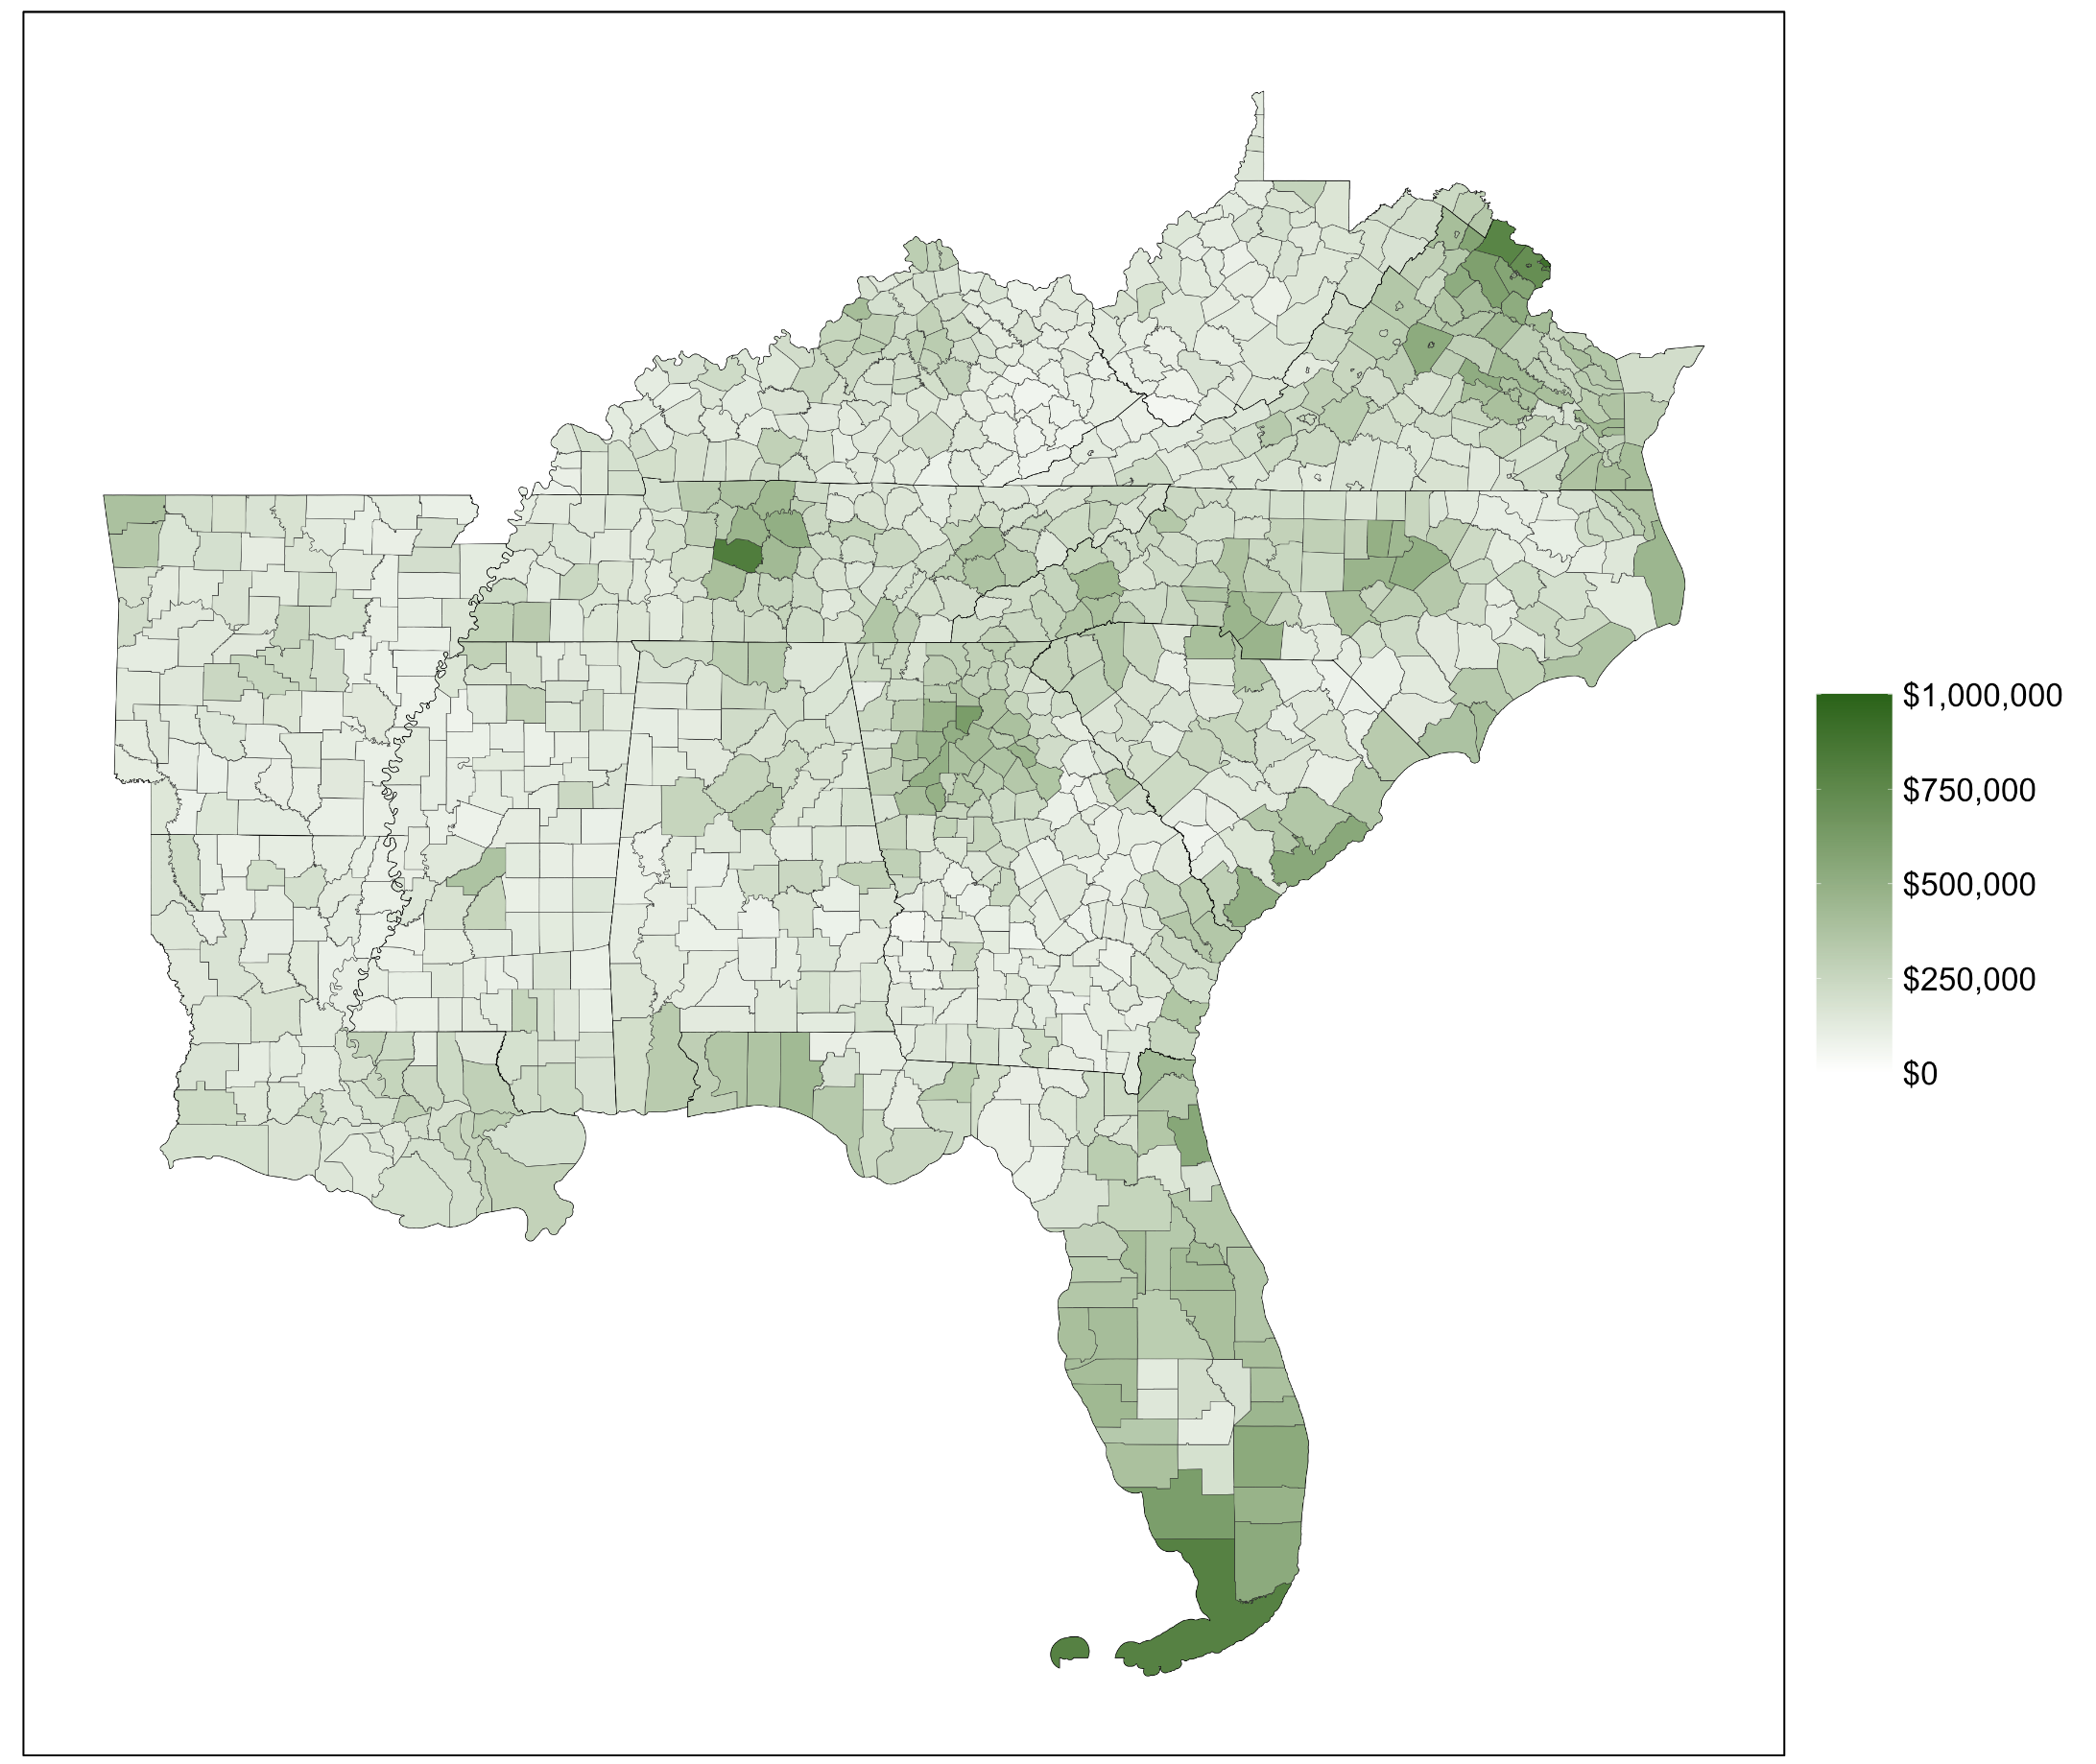
\includegraphics[width=0.85\textwidth]{fig1.png}
  \caption{\textbf{County Median Home Prices Q3 2024}\\\textit{Southeastern United States}}
  \label{fig:figure1}
  \vspace{1ex}
  {\footnotesize\textit{Data Source: National Association of Realtors}}
\end{figure}
        	
In comparison, the Midwestern United States presents a different pattern shown within \textbf{Figure~\ref{fig:figure2}}. Areas around large urban centers such as Chicago, Minneapolis, and Columbus, show higher property values, but many Midwestern counties remain relatively affordable. The contrast between the Southeast and Midwest is striking and suggests that the Midwest has not experienced the same degree of housing price inflation as the Southeast within the past 20 years. A county’s proximity to large urban centers is likely to inflate its housing costs, and this trend is studied further with several datasets present in this paper.  

%%%%%% FIGURE 2
\begin{figure}[H]
  \centering
  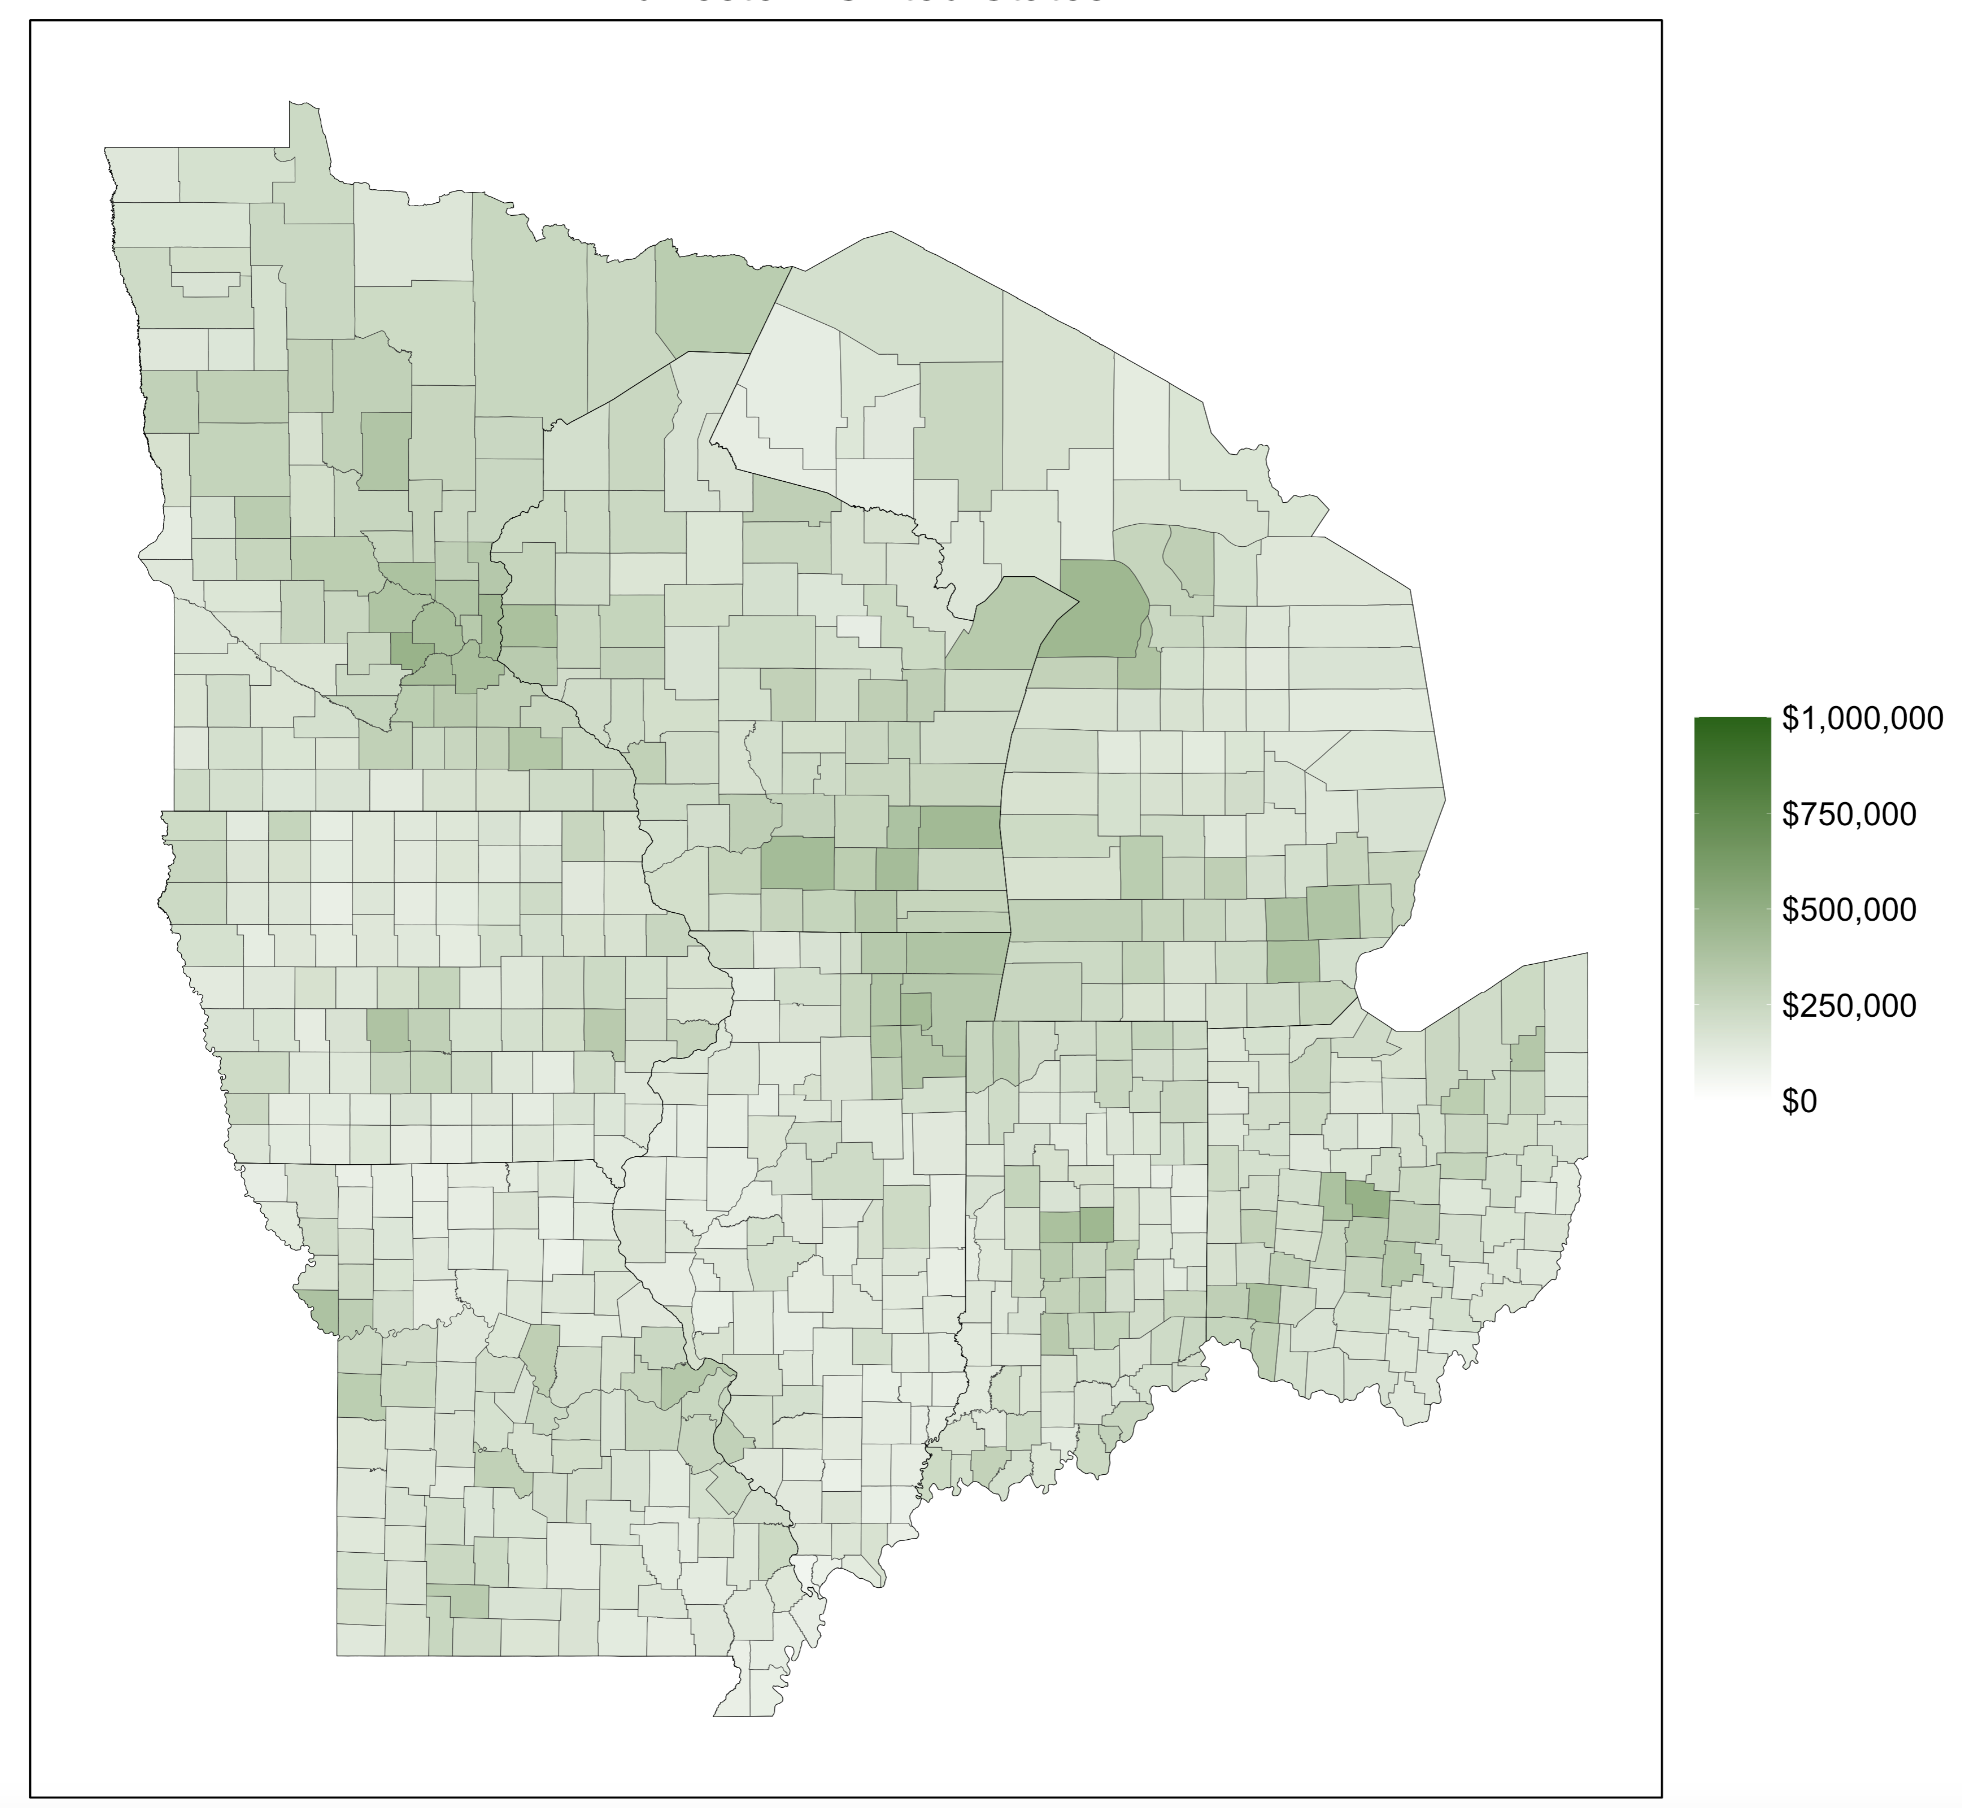
\includegraphics[width=0.85\textwidth]{fig2.png}
  \caption{\textbf{County Median Home Prices Q3 2024}\\\textit{Midwestern United States}}
  \label{fig:figure2}
  \vspace{1ex}
  {\footnotesize\textit{Data Source: National Association of Realtors}}
\end{figure}

\textbf{Figure~\ref{fig:figure3}} provides a combined view of the two regions, further emphasizing regional differences on one plot. The affordability of housing remains notably higher in the Midwest compared to the Southeast. This aligns within broader trends in regional growth patterns, where the Southeast has experienced greater population inflow and growth than the Midwest. These trends are later explored further within this research, and can be viewed within \textbf{Figure~\ref{fig:figure13}}, \textbf{Figure~\ref{fig:figure14}}, and \textbf{Figure~\ref{fig:figure15}}.

\begin{comment}
\textcolor{red}{
\textbf{Figure~\ref{fig:figure3}} provides a combined view of the two regions, further emphasizing regional differences on one plot. The affordability of housing remains notably higher in the Midwest compared to the Southeast. This aligns within broader trends in regional growth patterns, where the Southeast has experienced greater population inflow and growth than the Midwest. These trends are later explored further within this research, and can be viewed within \textbf{Figure~\ref{fig:figure13}}, \textbf{Figure~\ref{fig:figure14}}, and \textbf{Figure~\ref{fig:figure15}}.
}
\end{comment}

%%%%%% FIGURE 3
\begin{figure}[H]
  \begin{adjustwidth}{-\extralength}{0cm}
    \centering
    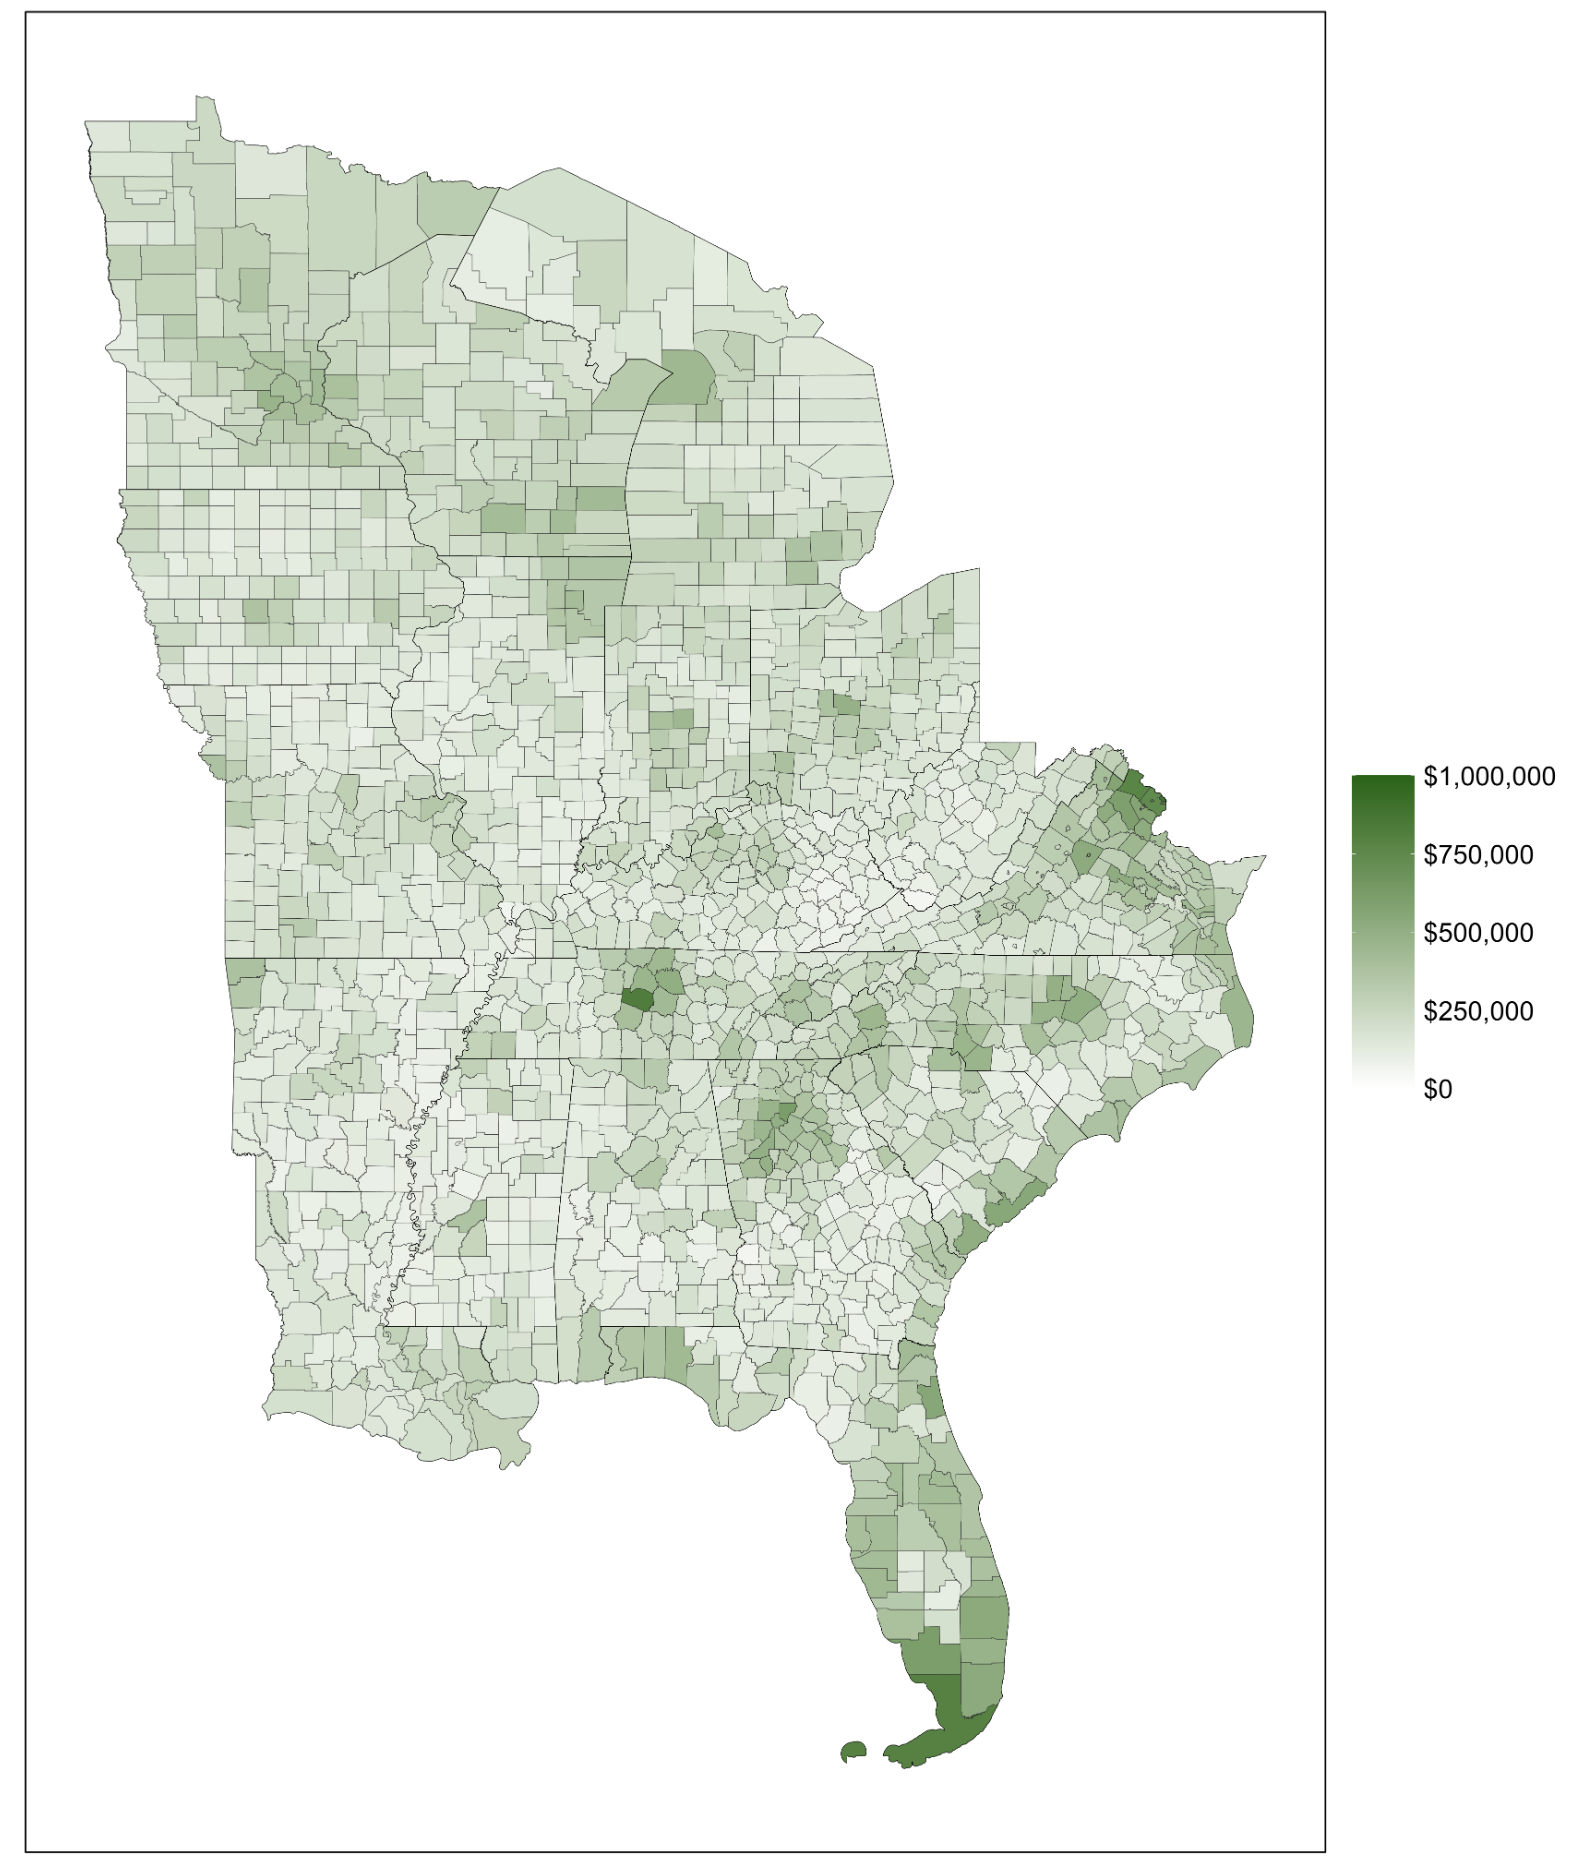
\includegraphics[width=\fulllength]{fig3.png}
    \caption{\textbf{County Median Home Prices Q3 2024}\\\textit{Combined Southeastern and Midwestern United States}}
    \label{fig:figure3}
    \vspace{1ex}
    {\footnotesize\textit{Data Source: National Association of Realtors}}
  \end{adjustwidth}
\end{figure}

\vspace{5cm}

An analysis of historical Housing Price Index (HPI) data provides further context for these findings, with the data being sourced from the Federal Reserve Bank of St. Louis \citep{a2024_hpi}. \textbf{Figure~\ref{fig:figure4}} compares the historical HPI for these regions and shows that while both have seen steady growth over time, the Southeast has experienced a steeper increase in housing prices after the economic crisis of 2008. This aligns with recent population shifts to the southeastern region. Additionally, ARIMA forecasting models predict housing price index trends through 2030. The forecasts within \textbf{Figure~\ref{fig:figure5}} indicate that housing prices in both regions are expected to rise, however the Southeast is predicted to experience slightly higher price acceleration over time. The confidence intervals highlight potential variability within the data and forecasting model and outline the uncertainty of economic conditions in the coming years.

%%%%%% FIGURES 4 and 5
\begin{figure}[H]
  \centering
  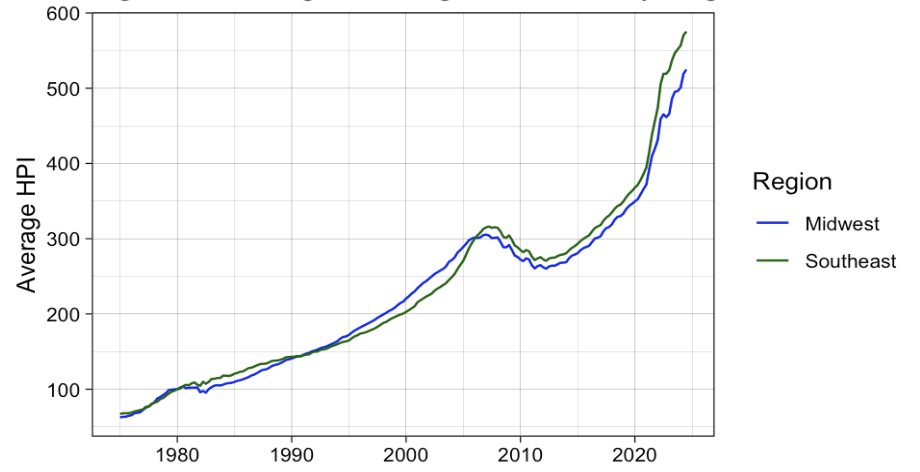
\includegraphics[width=0.85\textwidth]{fig4.png}
  \caption{\textbf{Average Housing Price Index by Region (1975–2024)}\\\textit{Midwest vs Southeast}}
  \label{fig:figure4}
  \vspace{1ex}
  {\footnotesize\textit{Data Source: Federal Reserve Bank of St. Louis}}
\end{figure}

\begin{figure}[H]
  \centering
  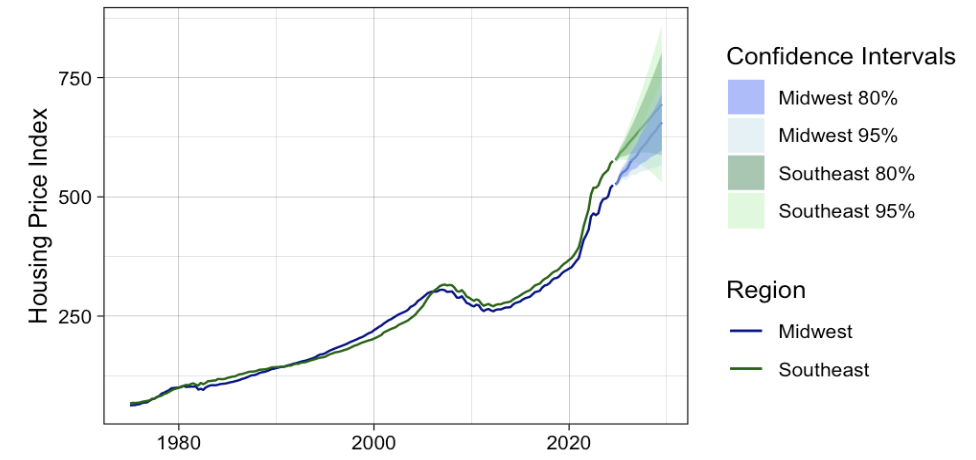
\includegraphics[width=0.85\textwidth]{fig5.png}
  \caption{\textbf{ARIMA Forecast of Housing Price Index by Region}\\\textit{Historical and Predicted Data (Quarterly)}}
  \label{fig:figure5}
  \vspace{1ex}
  {\footnotesize\textit{Data Source: Federal Reserve Bank of St. Louis}}
\end{figure}

To provide further detail for these models, \textbf{Table~\ref{tab:table2}} presents the forecasted HPI values, and includes lower and upper confidence intervals at 80\% and 95\% levels. These projections suggest that, while both regions will see growth, the Midwest remains slightly more stable than the Southeast within housing affordability. \textbf{Table~\ref{tab:table2}} shows a summary of these forecasts and outlines key statistics such as the mean predicted HPI, as well as the specific ARIMA models that are used within the forecasts.

%%%%%% TABLE 2 %%%%%%
\begin{table}[H]
\caption{Summary of Housing Price Index ARIMA Forecasts (1975–2030)\label{tab:table2}}
\begin{adjustwidth}{-\extralength}{0cm}
\begin{tabularx}{\fulllength}{@{}>{\raggedright\arraybackslash}p{1.6cm} >{\raggedright\arraybackslash}p{2.2cm} >{\centering\arraybackslash}p{1.5cm} >{\centering\arraybackslash}p{1.9cm} >{\centering\arraybackslash}p{1.9cm} >{\centering\arraybackslash}p{1.8cm} >{\centering\arraybackslash}p{2.2cm} >{\centering\arraybackslash}X@{}}
\toprule
\textbf{Region} & \textbf{ARIMA Model} & \textbf{Latest HPI} & \textbf{Forecast Start} & \textbf{Forecast End} & \textbf{Mean HPI} & \textbf{80\% CI Bounds} & \textbf{95\% CI Bounds} \\
\midrule
Midwest & ARIMA(0,2,2) & 524.85 & 2024-10-01 & 2026-07-01 & 552.24 & 540.49–563.98 & 534.27–570.20 \\
Southeast & ARIMA(2,2,0) & 575.28 & 2024-10-01 & 2026-07-01 & 600.37 & 584.31–616.44 & 575.81–624.94 \\
\bottomrule
\end{tabularx}
\end{adjustwidth}
\noindent{\footnotesize \textit{Source: Federal Reserve Bank of St. Louis (FRED).}}
\end{table}
%%%%%% TABLE 2 %%%%%%

The ARIMA (AutoRegressive Integrated Moving Average) models used in this analysis were specifically selected by using the \texttt{auto.arima()} function within the \texttt{forecast} package in R and RStudio. This allowed for automatic evaluation of models across combinations of different parameters, and a final selection of the model which minimized the Akaike Information Criterion -- AIC.  
\begin{itemize}
    \item The Midwest’s ARIMA(0,2,2) model indicates a series with a strong trend component, and a higher reliance on moving average terms which were used to capture any short term fluctuations in the data.
    \item The Southeast’s ARIMA(2,2,0) model incorporates autoregressive terms, which suggests that the housing prices within its model are more influenced by past values and exhibit more behavior driven by past momentum. This matches the outputs provided by previous figures as there are more clusters of higher income areas within the Southeastern United States, which may drive trends within the region.
\end{itemize}

\textbf{Figure~\ref{fig:figure5}} shows a clearer comparison of historical and projected HPI values by region, and includes shaded confidence intervals that show uncertainty levels in the projection. The expected outcomes include more stable price fluctuations in the Midwest, and more volatile but potentially greater growth within the Southeast.

The Zillow Housing Dataset further supports these findings by offering a county-level view of home price estimates, using Zillow specific data \citep{zillow_2024_housing}. \textbf{Figure~\ref{fig:figure6}} presents a scatterplot of Zillow’s home price index estimates over time and shows a general upward trend. Notably, however, home values in the Southeastern region trend in a more volatile manner and align with the observed patterns from the HPI dataset. An ARIMA forecast was used with this data as well, and the Zillow data mirrors the Housing Price Index trend of upward trajectory through 2030, particularly in the Southeast.

%%%%%% FIGURE 6
\begin{figure}[H]
  \centering
  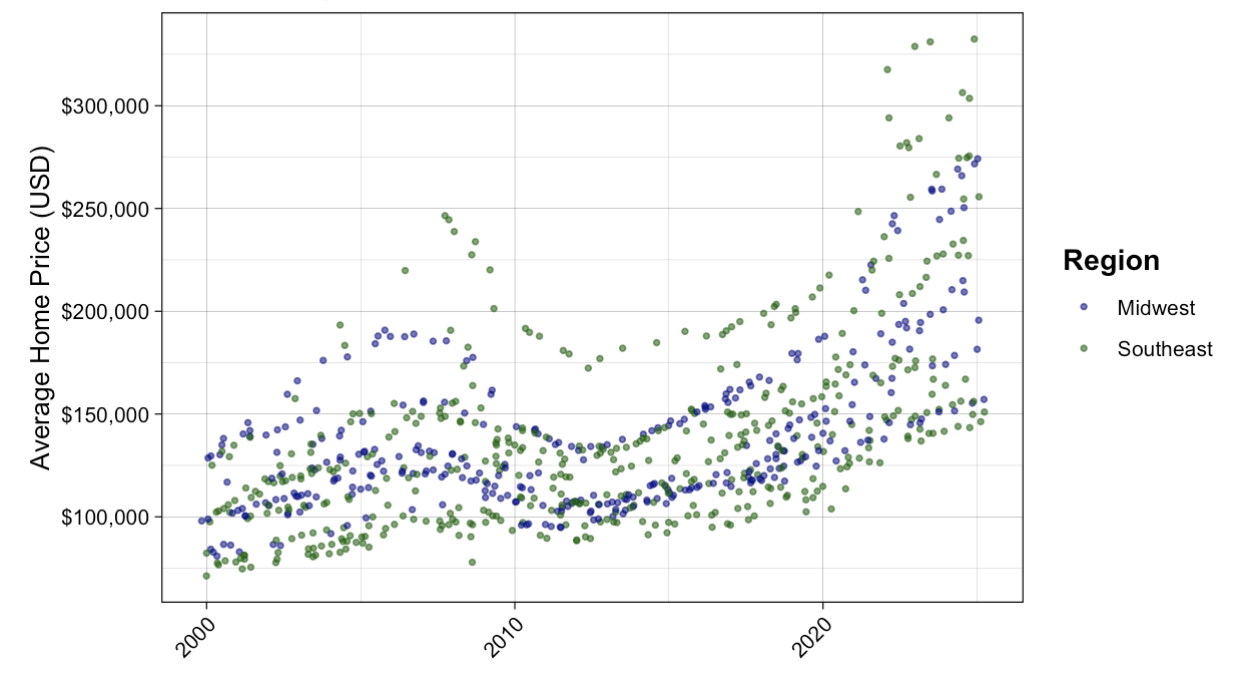
\includegraphics[width=0.85\textwidth]{fig6.png}
  \caption{\textbf{Zillow Home Price Estimates by State}\\\textit{Random Sample from Zillow Data}}
  \label{fig:figure6}
  \vspace{1ex}
  {\footnotesize\textit{Data Source: Zillow Research}}
\end{figure}

The ARIMA models summarized in \textbf{Table~\ref{tab:table3}} were also chosen using the \texttt{auto.arima()} function from the \texttt{forecast} package in R and RStudio, similar to \textbf{Table~\ref{tab:table2}}. This allowed for the evaluation of multiple models, and the selection of the model with the smallest AIC value. In this table, the Midwestern model utilized an ARIMA(3,2,0) model, while an ARIMA(2,2,2) model was used for the Southeast. These two models allowed for thorough forecasting for each region and can be seen in \textbf{Figure~\ref{fig:figure7}}. 

%%%%%% TABLE 3 %%%%%%
\begin{table}[H]
\caption{Summary of Zillow Home Price Index ARIMA Forecasts (2025–2029)\label{tab:table3}}
\begin{adjustwidth}{-\extralength}{0cm}
\small % Reduce font size
\begin{tabularx}{\fulllength}{@{}>{\raggedright\arraybackslash}p{1.6cm} >{\raggedright\arraybackslash}p{2.2cm} >{\centering\arraybackslash}p{1.5cm} >{\centering\arraybackslash}p{1.9cm} >{\centering\arraybackslash}p{1.9cm} >{\centering\arraybackslash}p{1.8cm} >{\centering\arraybackslash}p{2.2cm} >{\centering\arraybackslash}X@{}}
\toprule
\textbf{Region} & \textbf{ARIMA Model} & \textbf{Latest HPI} & \textbf{Forecast Start} & \textbf{Forecast End} & \textbf{Mean ZHPI} & \textbf{80\% CI Bounds} & \textbf{95\% CI Bounds} \\
\midrule
Midwest & ARIMA(3,2,0) & 210{,}837 & 2025-04-01 & 2029-01-01 & 229{,}559 & 212{,}806–246{,}313 & 203{,}937–255{,}182 \\
Southeast & ARIMA(2,2,2) & 223{,}193 & 2025-04-01 & 2029-01-01 & 239{,}959 & 217{,}163–262{,}755 & 205{,}096–274{,}823 \\
\bottomrule
\end{tabularx}
\end{adjustwidth}
\noindent{\footnotesize \textit{Source: Zillow Research (2024). Data uses Zillow’s Housing Price Index – Zillow Home Value Index (ZHVI).}}\\
\noindent{\footnotesize \textit{Note: All Zillow HPI values are in U.S. dollars (USD).}}
\end{table}
%%%%%% TABLE 3 %%%%%%

%%%%%% FIGURE 7
\begin{figure}[H]
  \centering
  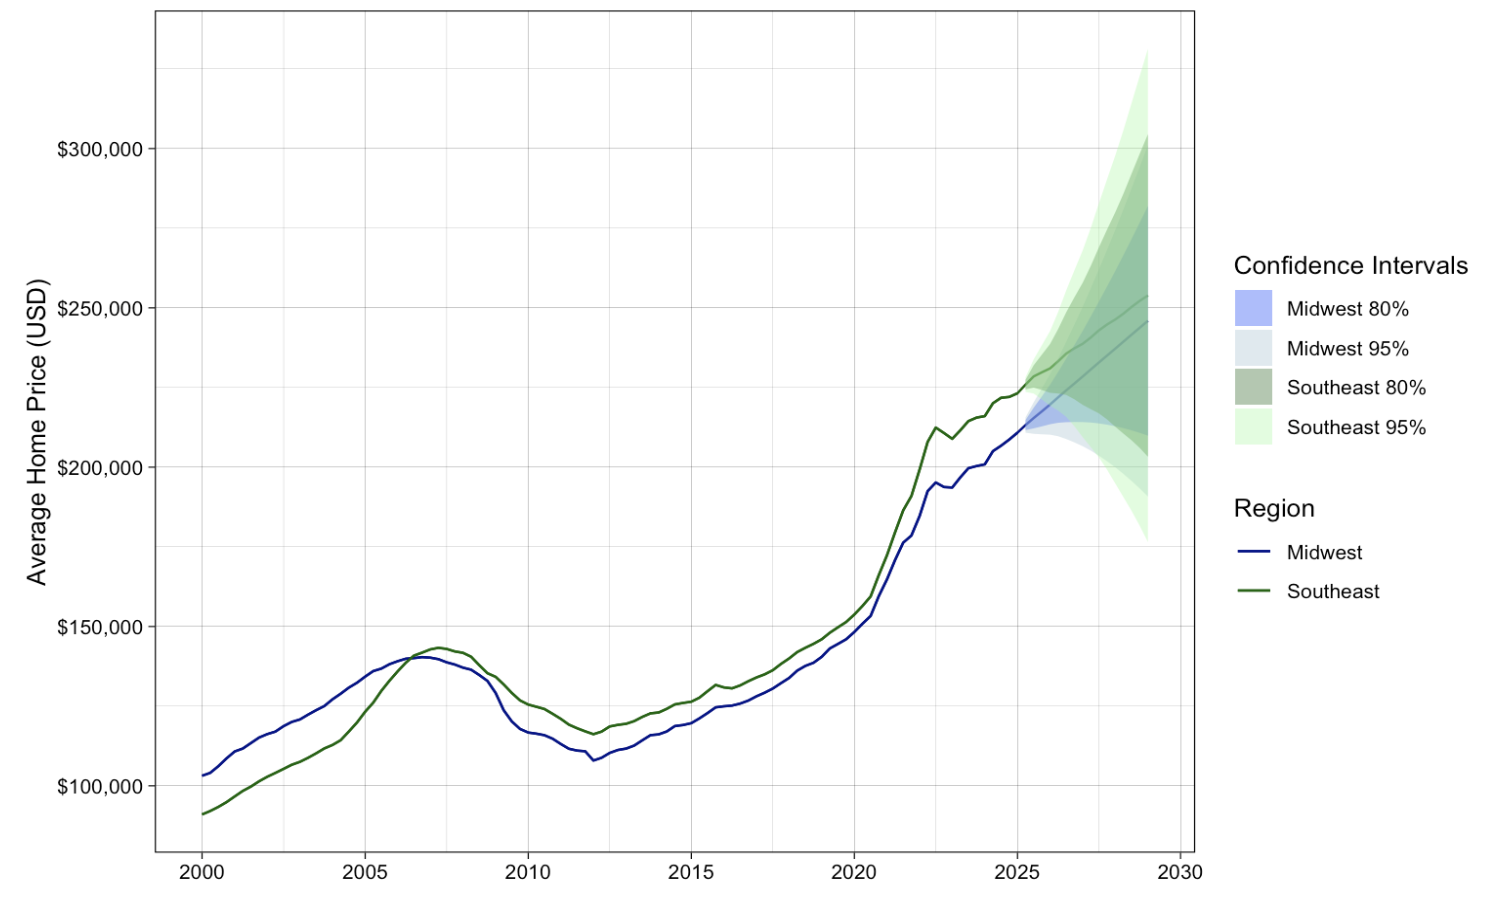
\includegraphics[width=0.85\textwidth]{fig7.png}
  \caption{\textbf{ARIMA Forecast of Zillow Home Price Estimates}\\\textit{Historical and Predicted Data (Quarterly)}}
  \label{fig:figure7}
  \vspace{1ex}
  {\footnotesize\textit{Data Source: Zillow Research}}
\end{figure}

These specific models reflect how each region has experienced changing housing prices over time, with the Midwest seeing a more autoregressive pattern with additional differencing, and the Southeast seeing both autoregressive and moving-average components, which reveals more complex price dynamics within the region.

The Zillow Research data introduces a certain level of bias, as Zillow’s metrics are proprietary and could emphasize different aspects of housing valuation in comparison to the HPI utilized in the previous ARIMA model \citep{zillow_2024_housing}. Despite this, the Zillow data provides more granular coverage of local trends and provides a more interpretable forecast, including average home values instead of a standardized index. Through these visuals and tables, it is apparent that the Southeastern region of the United States is experiencing higher volatility with a steeper growth projection than that of the Midwestern United States, which mirrors the results found in previous figures and forecasts.

\subsection{Analysis}

The preliminary findings from this analysis suggest that there is a significant relationship between population dynamics and housing price trends in the Southeastern and Midwestern United States. While these findings focus primarily on housing prices and historical housing data, this research is expanded through hedonic regression modeling and panel data estimation, to directly compare the impacts of population density and population growth with housing prices. The choropleth maps highlight the stark contrast in housing affordability within the two regions, and the historical and forecasted Housing Price Index trends reinforce these metrics, indicating that the Southeast will likely continue to see higher price growth relative to the Midwest through 2030. The ARIMA forecasting models provide a valuable tool to predict future trends, and this methodology can be used to predict future housing trends for both regions in addition to housing price metrics. This aligns with broader economic patterns, as increased population migration, business expansion, and labor market shifts continue to shape housing demands. The next steps within this research will consist of:

\begin{itemize}
    \item \textbf{Hedonic Price Modeling} \\
    Incorporates data from the National Association of Realtors and United States Census Bureau, and focuses on effects of population growth and density on housing prices.

    \item \textbf{Panel Data Estimation} \\
    Fixed Effects or Random Effects Panel Model implementation. \\
    Analyzes how regional and time-specific factors drive price movements.
\end{itemize}

The initial results demonstrate that population density and growth play a crucial role in shaping housing markets across these regions in the United States, and the next stages of this research will refine these findings and provide more finite results to inform housing market strategies, affordability policies, and urban development planning.

In addition to modeling future housing price trends, understanding the current demographics of the United States is essential to evaluate the results from this data. To explore these factors, this section provides a series of spatial and statistical visualizations to examine the relationship between population trends in certain areas with housing prices in both the Southeastern and Midwestern United States.

\textbf{Figure~\ref{fig:figure8}} illustrates county-level population estimates in 2023 using data from the United States Census Bureau \citep{_2023_county}. This directly compares both regions and draws attention to certain urban centers, namely Cook County in Illinois (Chicago Area) and the Miami area within Florida. Zoomed-in maps allow for greater detail to be seen within the population differences and are present within \textbf{Figure~\ref{fig:figure9}} (Greater Chicago Area) and \textbf{Figure~\ref{fig:figure10}} (Florida Area). This provides a closer analysis of any regional hot-spots that are available in each region and show certain outliers that could drive trends in either region. This emphasizes the population distribution of each region and points toward corresponding disparities within housing demand in each region, and the corresponding housing price growth over time.

%%%%%% FIGURES 8, 9, 10

\begin{figure}[H]
  \begin{adjustwidth}{-\extralength}{0cm}
    \centering
    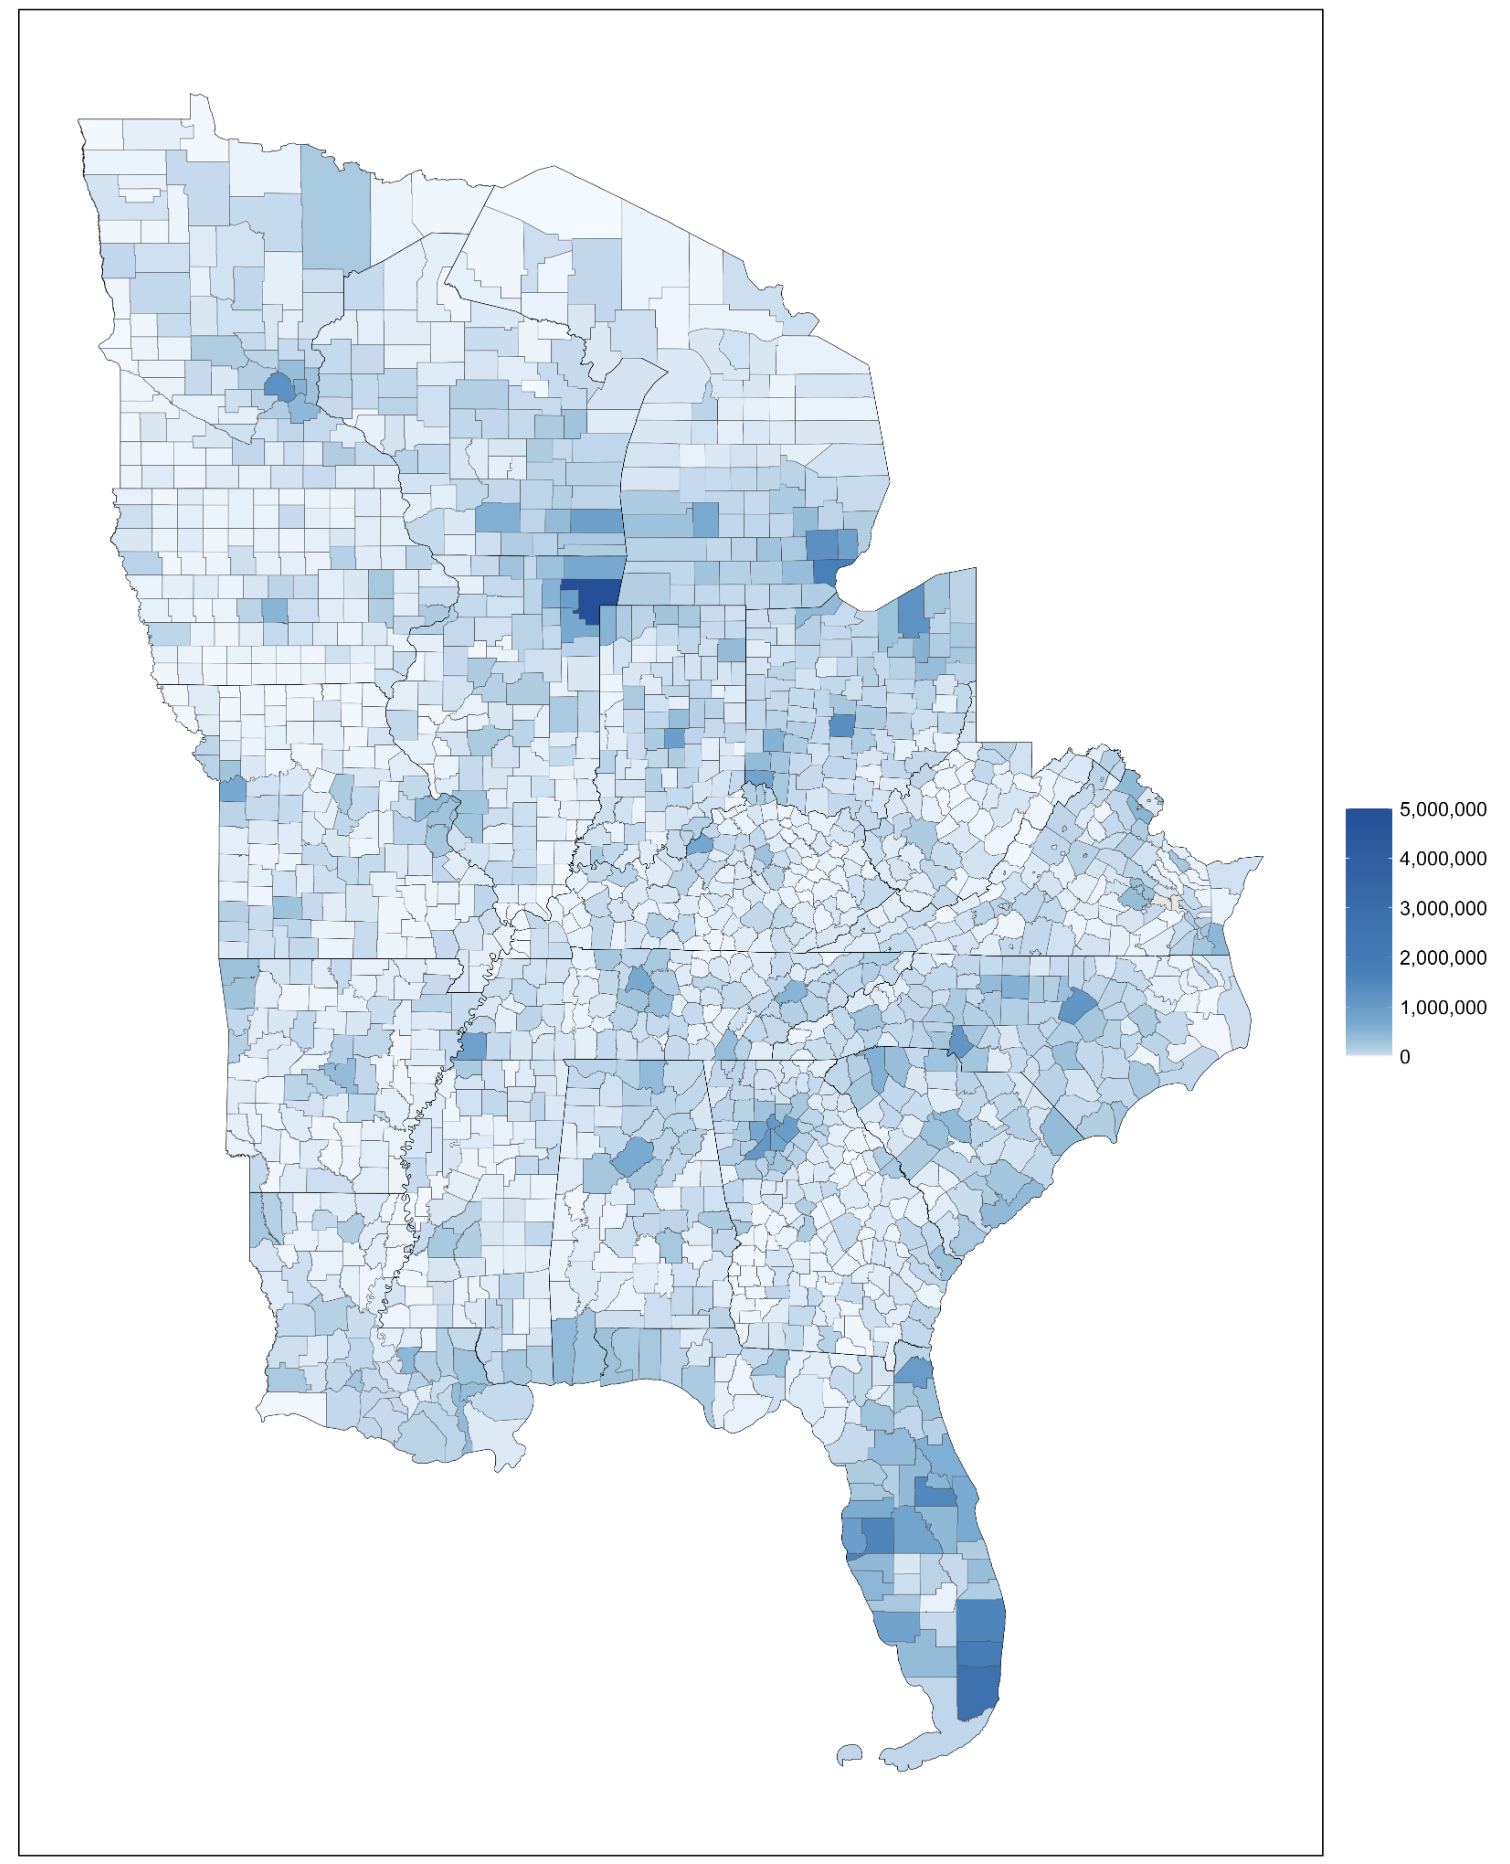
\includegraphics[width=\fulllength]{fig8.png}
    \caption{\textbf{County Population Estimates (2023)}\\\textit{Southeastern and Midwestern United States}}
    \label{fig:figure8}
    \vspace{1ex}
    {\footnotesize\textit{Data Source: U.S. Census Bureau}}
  \end{adjustwidth}
\end{figure}

\begin{figure}[H]
  \centering
  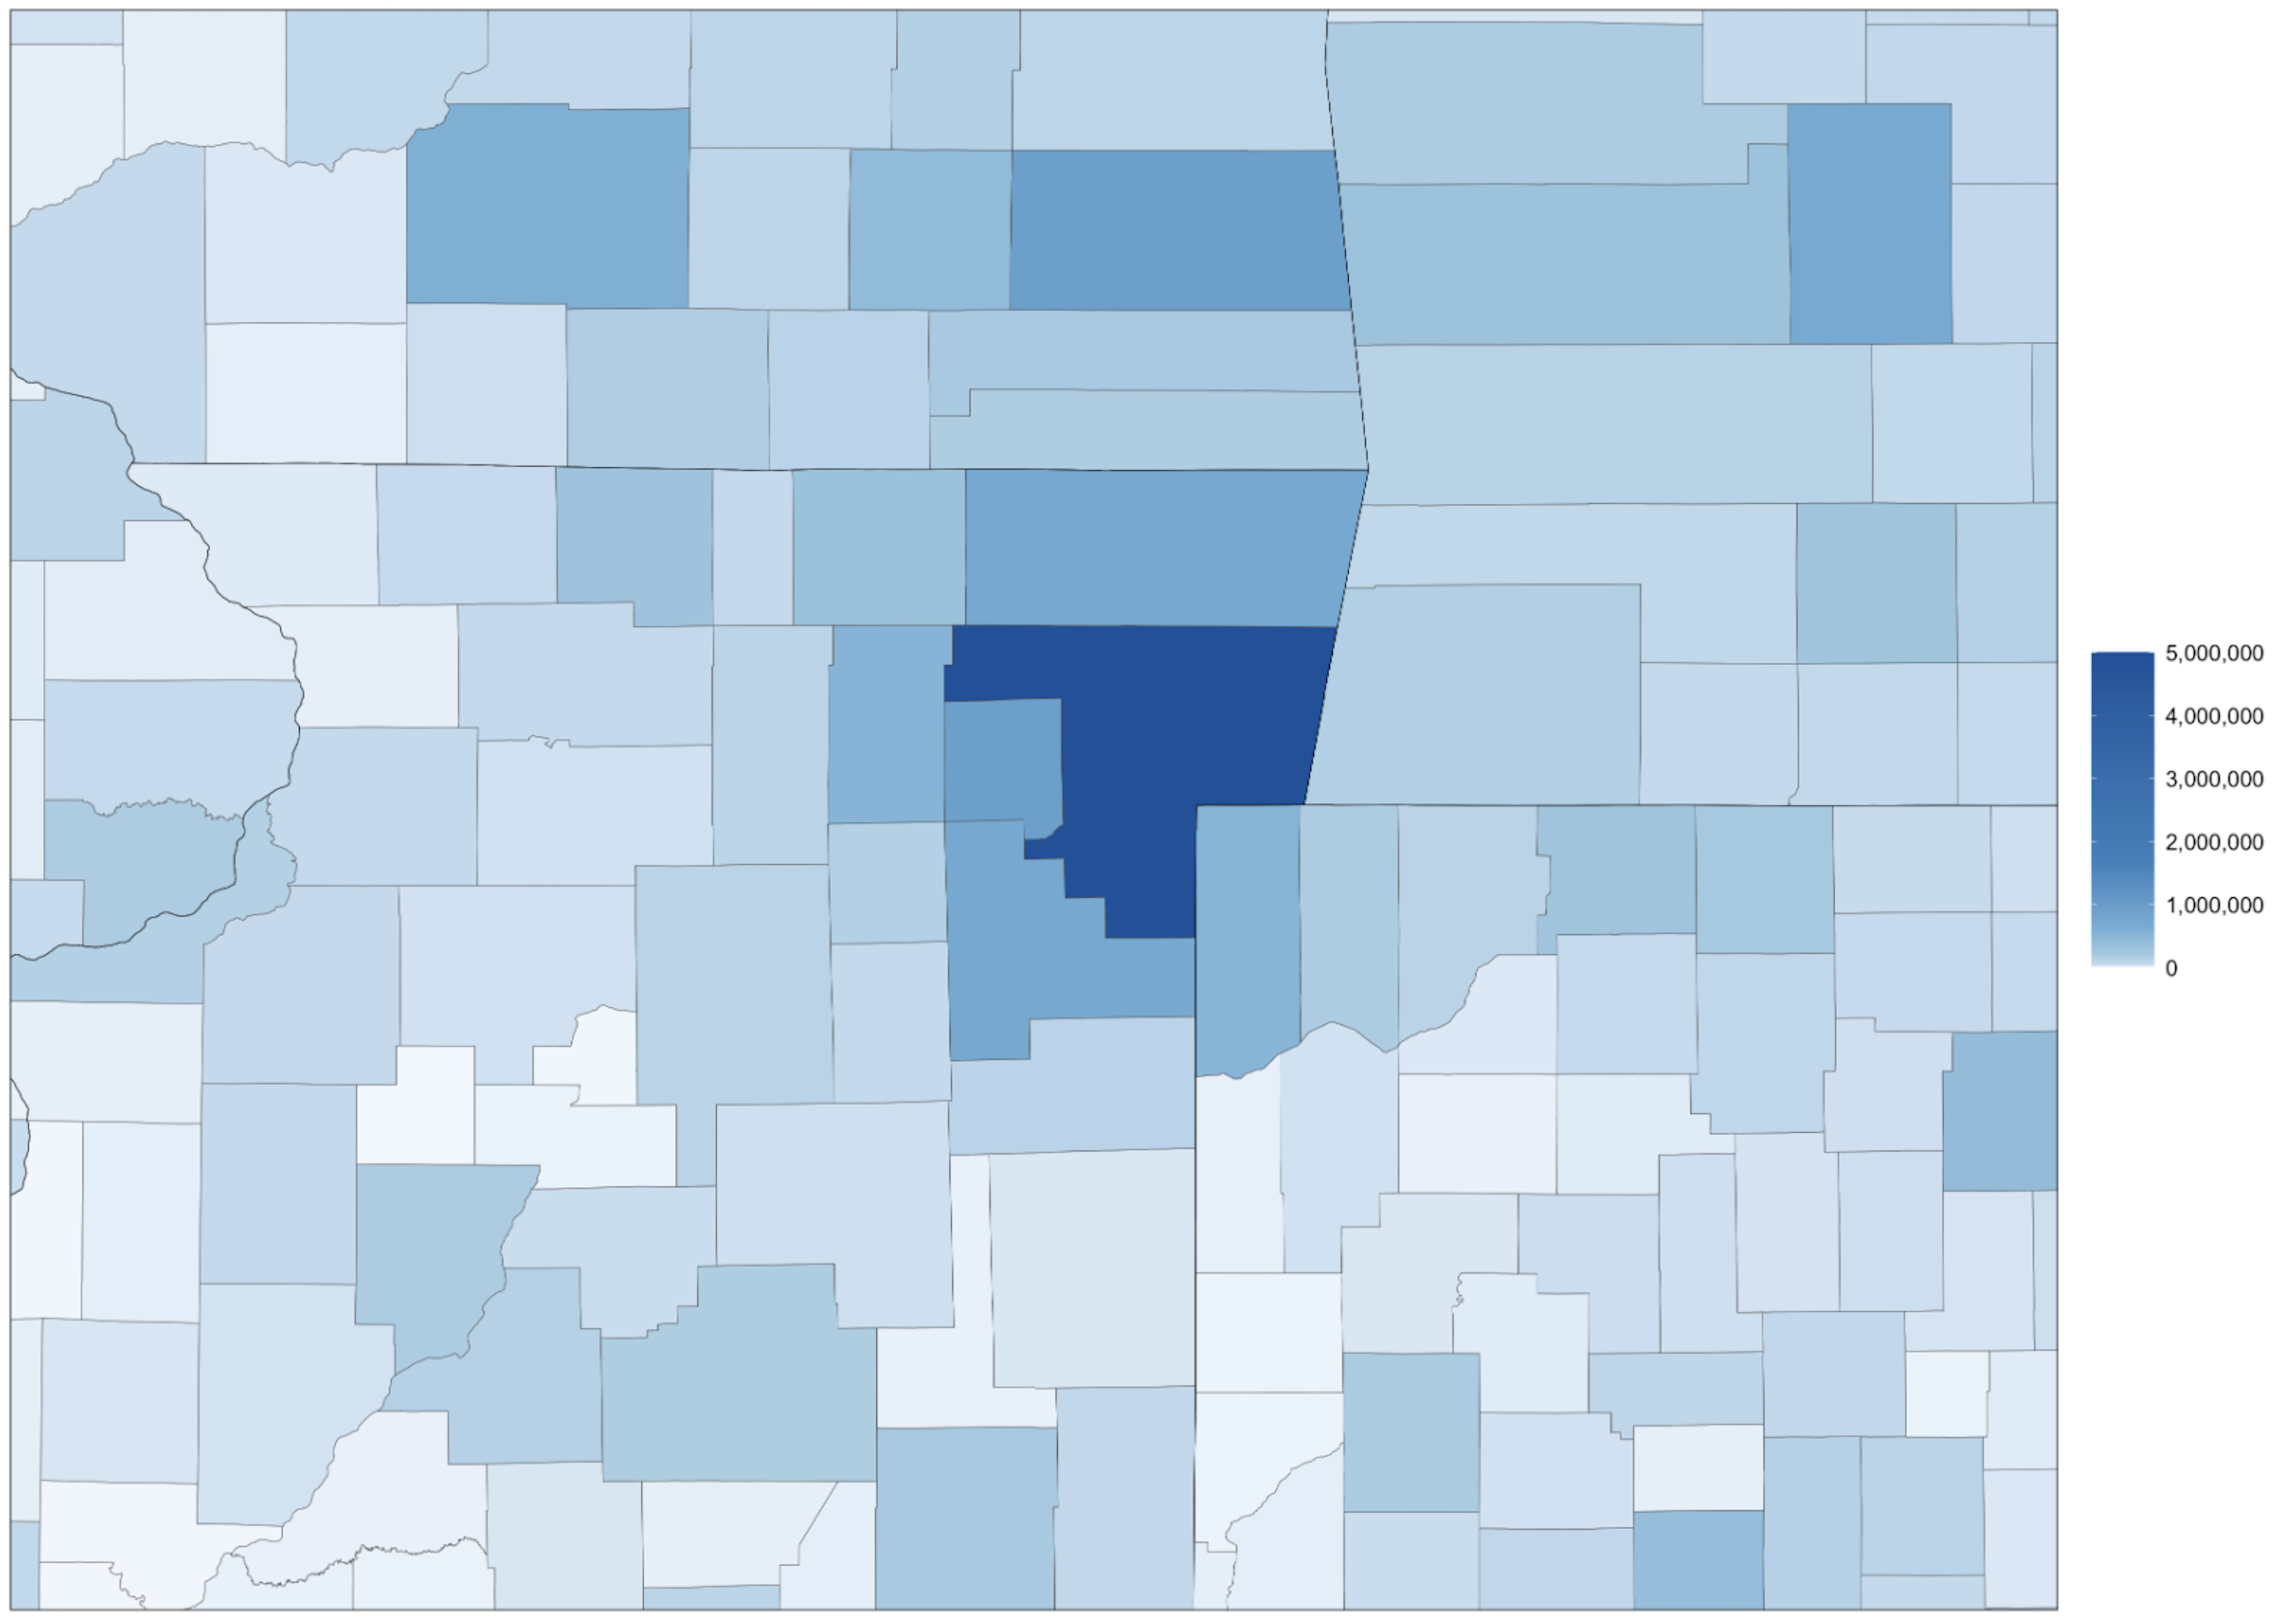
\includegraphics[width=0.85\textwidth]{fig9.png}
  \caption{\textbf{Cook County and Surrounding Population (2023)}\\\textit{Greater Chicago Area — Southeastern Wisconsin, Northern Indiana, and Northeast Illinois}}
  \label{fig:figure9}
  \vspace{1ex}
  {\footnotesize\textit{Data Source: U.S. Census Bureau}}
\end{figure}

\begin{figure}[H]
  \centering
  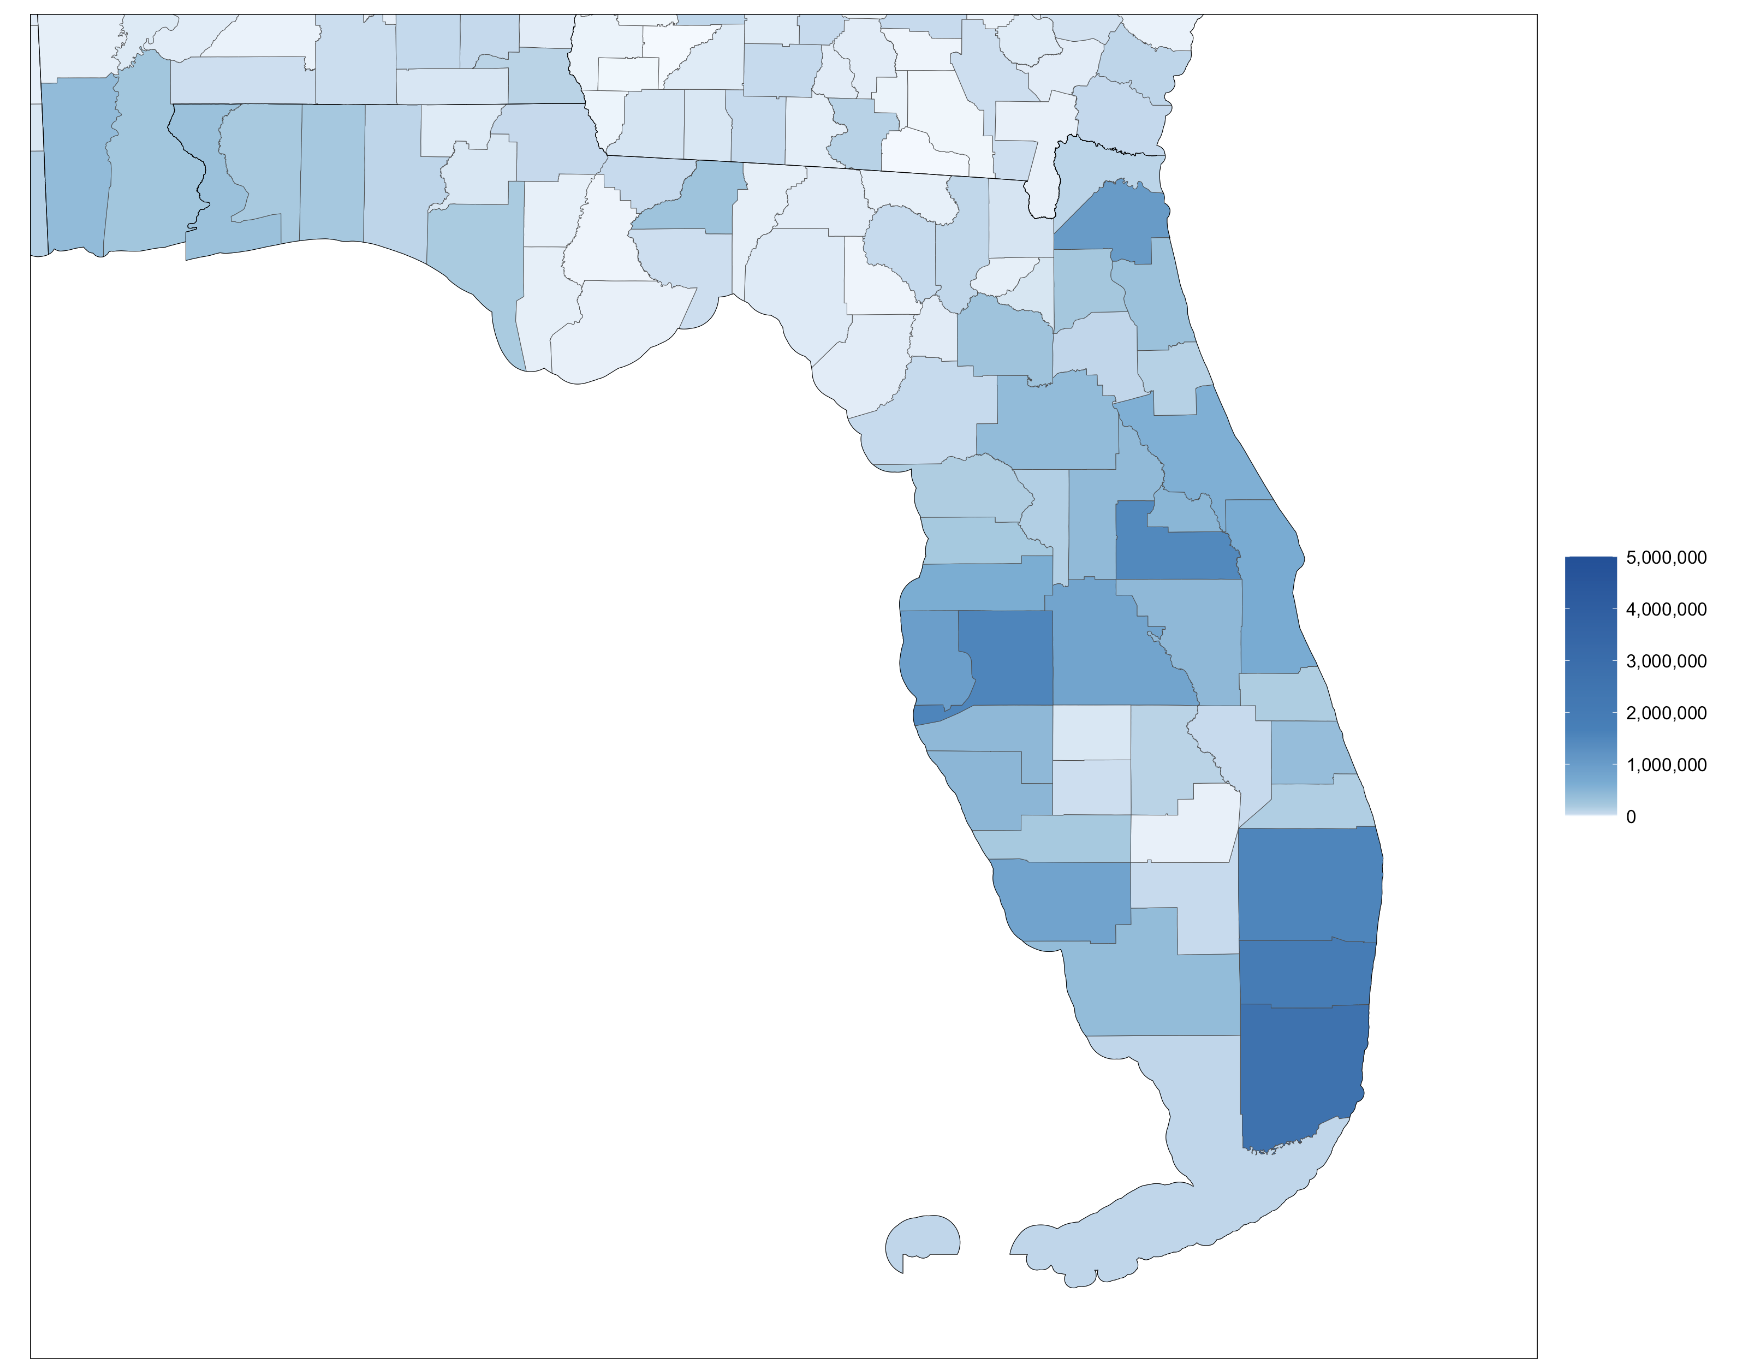
\includegraphics[width=0.85\textwidth]{fig10.png}
  \caption{\textbf{County Population Estimates (2023)}\\\textit{Florida Area}}
  \label{fig:figure10}
  \vspace{1ex}
  {\footnotesize\textit{Data Source: U.S. Census Bureau}}
\end{figure}

In addition to the analysis of the county-level population distribution in both regions, the Hedonic Pricing Model uses factors such as population size, mortgage payments, and state-specific fixed effects to understand different influences on housing prices. The state fixed effects allowed for further understanding of each explanatory variable. This hedonic model utilizes data from both the National Association of Realtors, as well as the United States Census Bureau to provide a thorough base for the model.

\begin{comment}
\textcolor{red}{
In addition to the analysis of the county-level population distribution in both regions, the Hedonic Pricing Model uses factors such as population size, mortgage payments, and state-specific fixed effects to understand different influences on housing prices. The state fixed effects allowed for further understanding of each explanatory variable. This hedonic model utilizes data from both the National Association of Realtors, as well as the United States Census Bureau to provide a thorough base for the model.
}
\end{comment}

\textbf{Table~\ref{tab:table4}} provides the output of the Hedonic Model, by studying the subset of Southeastern and Midwestern States used in this study. By using Alabama as a baseline reference category, \textbf{Table~\ref{tab:table4}} provides coefficients for the log of the 2023 population by county, average monthly payments from the third quarter of 2024, and individual states.

\begin{comment}
%%%%%% TABLE 4 %%%%%%
\begin{table}[H]
\caption{{\color{red}\textbf{Hedonic Model}\\
\small \textcolor{red}{Median Home Price $\sim$ log(Population), Mortgage Payment, State Fixed Effects}}\label{tab:table4}}
\begin{adjustwidth}{-\extralength}{0cm}
\small % Slightly smaller font for clarity
\begin{tabularx}{\fulllength}{@{}>{\raggedright\arraybackslash}p{3.5cm} >{\centering\arraybackslash}p{2.5cm} >{\centering\arraybackslash}p{3.8cm} >{\centering\arraybackslash}X@{}}
\toprule
\textbf{Variable} & \textbf{Beta} & \textbf{95\% CI} & \textbf{p-value} \\
\midrule
(Intercept) & -26 & -308, 257 & 0.9 \\
\texttt{log(pop\_2023)} & 8.3 & -19, 35 & 0.5 \\
\texttt{monthly\_payment\_q32024} & 176 & 176, 176 & <0.001 \\
\midrule
\textbf{Regional Fixed Effects (Summary)} & & & \\
Midwest (avg.) & -16.29 & 154, 43 & \\
Southeast (avg.) & -79.32 & 207, 19 & \\
\midrule
\textcolor{red}{\textbf{Model Fit}} & \textcolor{red}{$R^2 = 1.00$, Adj. $R^2 = 0.99997$} & \textcolor{red}{$N = 1793$} & \\
\bottomrule
\end{tabularx}
\end{adjustwidth}
\noindent{\footnotesize 
\textbf{Note:} This table summarizes the results of a hedonic regression model used to estimate median home prices across counties in the Southeastern and Midwestern U.S. The dependent variable is median home price, and the independent variables include the natural logarithm of 2023 population (\texttt{log(pop\_2023)}), the average monthly mortgage payment in Q3 2024 (\texttt{monthly\_payment\_q32024}), and state-level fixed effects. Rather than listing all state coefficients, average fixed effects are shown by region. Coefficients (Beta) represent the estimated change in median home price (in USD) associated with a one-unit change in the predictor, holding other variables constant. Confidence intervals (95\% CI) indicate the estimated range of the true coefficient. The CI ranges shown for the regional effects are aggregated summaries for reference only and are not derived directly from the model output. \\
\textbf{Model fit:} The high $R^2$ reflects the inclusion of state fixed effects and the low variance in mortgage payments across counties. \\
\textbf{Data Source:} National Association of Realtors, United States Census Bureau.
}
\end{table}
%%%%%% TABLE 4 %%%%%%
\end{comment}

%%%%%% TABLE 4 %%%%%%
\begin{table}[H]
\caption{\textbf{Hedonic Model}\\
\small Median Home Price $\sim$ log(Population), Mortgage Payment, State Fixed Effects\label{tab:table4}}
\begin{adjustwidth}{-\extralength}{0cm}
\small % Slightly smaller font for clarity
\begin{tabularx}{\fulllength}{@{}>{\raggedright\arraybackslash}p{3.5cm} >{\centering\arraybackslash}p{2.5cm} >{\centering\arraybackslash}p{3.8cm} >{\centering\arraybackslash}X@{}}
\toprule
\textbf{Variable} & \textbf{Beta} & \textbf{95\% CI} & \textbf{p-value} \\
\midrule
(Intercept) & -26 & -308, 257 & 0.9 \\
\texttt{log(pop\_2023)} & 8.3 & -19, 35 & 0.5 \\
\texttt{monthly\_payment\_q32024} & 176 & 176, 176 & <0.001 \\
\midrule
\textbf{Regional Fixed Effects (Summary)} & & & \\
Midwest (avg.) & -16.29 & 154, 43 & \\
Southeast (avg.) & -79.32 & 207, 19 & \\
\midrule
\textbf{Model Fit} & $R^2 = 1.00$, Adj. $R^2 = 0.99997$ & $N = 1793$ & \\
\bottomrule
\end{tabularx}
\end{adjustwidth}
\noindent{\footnotesize 
\textbf{Note:} This table summarizes the results of a hedonic regression model used to estimate median home prices across counties in the Southeastern and Midwestern U.S. The dependent variable is median home price, and the independent variables include the natural logarithm of 2023 population (\texttt{log(pop\_2023)}), the average monthly mortgage payment in Q3 2024 (\texttt{monthly\_payment\_q32024}), and state-level fixed effects. Rather than listing all state coefficients, average fixed effects are shown by region. Coefficients (Beta) represent the estimated change in median home price (in USD) associated with a one-unit change in the predictor, holding other variables constant. Confidence intervals (95\% CI) indicate the estimated range of the true coefficient. The CI ranges shown for the regional effects are aggregated summaries for reference only and are not derived directly from the model output. \\
\textbf{Model fit:} The high $R^2$ reflects the inclusion of state fixed effects and the low variance in mortgage payments across counties. \\
\textbf{Data Source:} National Association of Realtors, United States Census Bureau.
}
\end{table}
%%%%%% TABLE 4 %%%%%%

The model indicates that monthly mortgage payment is the most significant method of predicting median home price, with a coefficient of 176 and a p-value less than 0.001. This represents that for every dollar increase in monthly mortgage payments, the median home price rises by approximately 176 USD. This result is highly significant and relevant to the study at hand, and these results are expected as areas with higher mortgage payments are likely to have more expensive housing options.

Another result derived from \textbf{Table~\ref{tab:table4}} is the coefficient for the logged Population variable, because it is positive (8.3), yet not statistically significant with a p-value equaling 0.5. This is unexpected as a higher population could be used to predict increasing housing demand, and therefore higher housing prices. However, the results within this model suggest that population size alone does not have a strong enough correlation on housing prices within the counties in these two regions. This might suggest that most population influences are already considered by state-specific dynamics or other economic factors. The data within this model was sourced by the National Association of Realtors and the United States Census Bureau \citep{_2024_county, _2023_county}.
 
By using Alabama as the reference state for both the Southeastern and Midwestern regions, it offers a balanced midpoint in terms of housing affordability for this research. Alabama had sufficient county-level observations and complete data for all key variables within the Hedonic model, therefore it was chosen over other states which may have had large outliers or missing data. It also provides an interesting reference point as it includes both rural and urban counties and is central to the Southeastern region.

The state fixed effects also provide significant results and are visualized within \textbf{Figure~\ref{fig:figure11}} and \textbf{Figure~\ref{fig:figure12}}. 

%%%%%% FIGURES 11, 12
\begin{figure}[H]
  \centering
  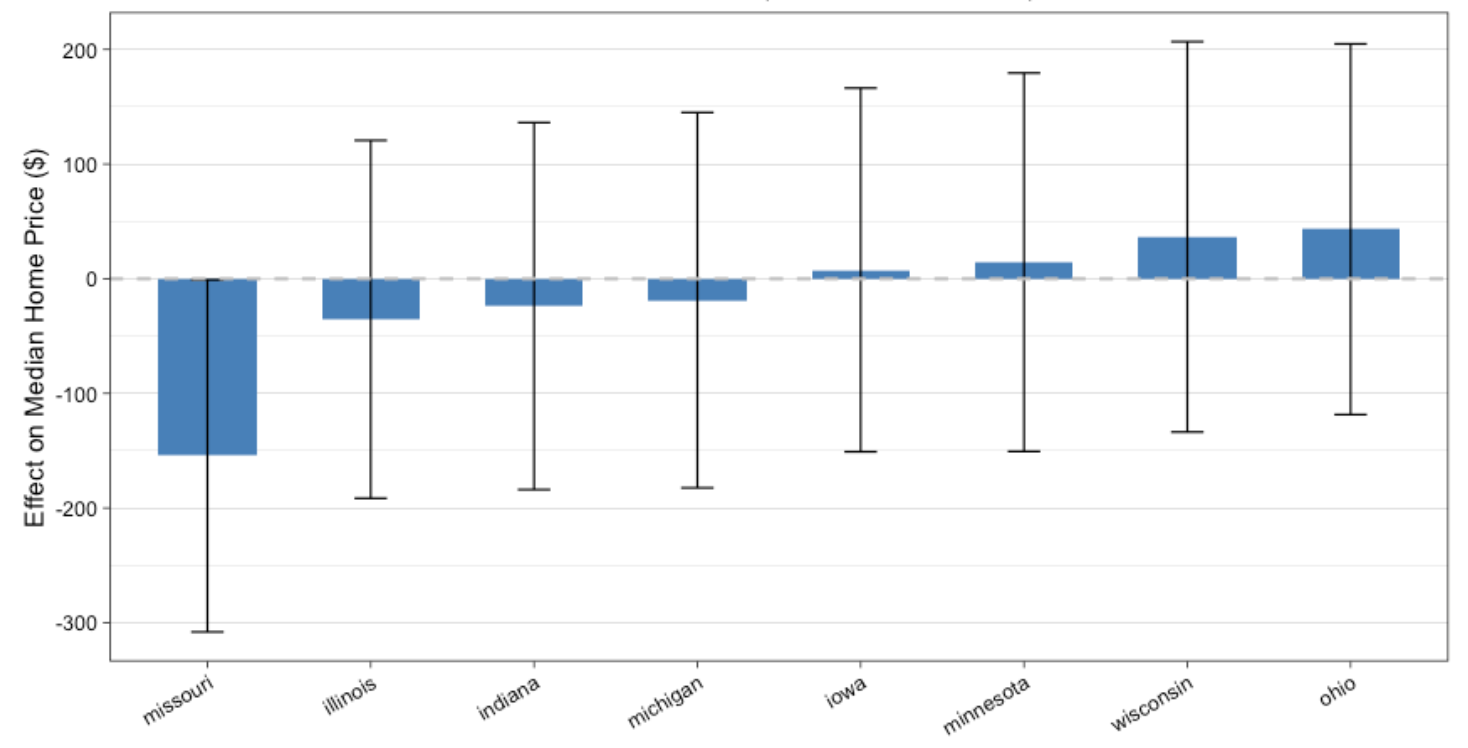
\includegraphics[width=0.95\textwidth]{fig11.png}
  \caption{\textbf{State Fixed Effects from Hedonic Model}\\\textit{Midwestern States (Reference: Alabama)}}
  \label{fig:figure11}
  \vspace{1ex}
  {\footnotesize\textit{Data Source: National Association of Realtors, United States Census Bureau}}
\end{figure}

\begin{figure}[H]
  \centering
  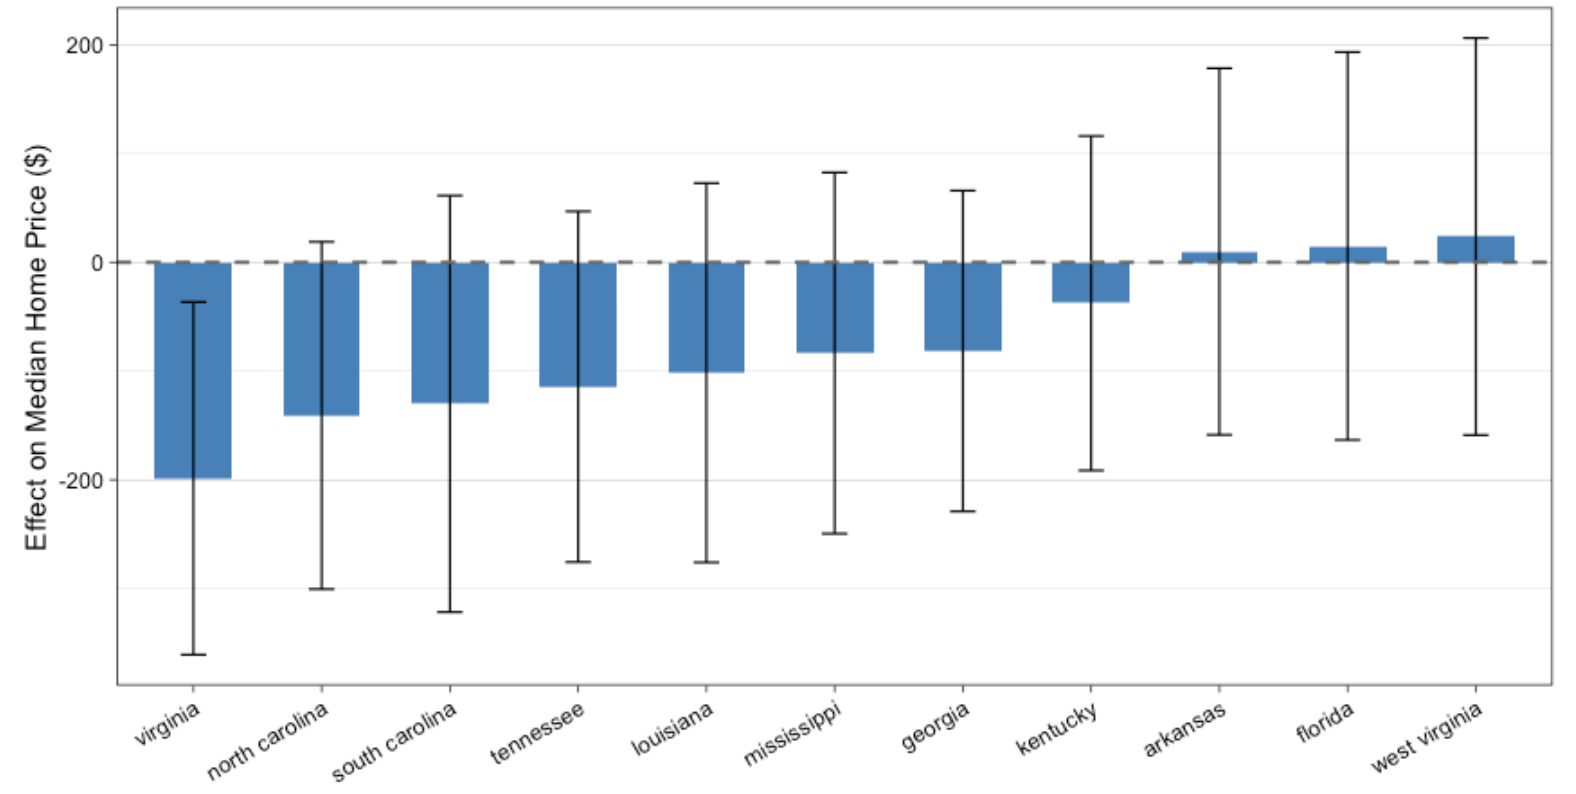
\includegraphics[width=0.95\textwidth]{fig12.png}
  \caption{\textbf{State Fixed Effects from Hedonic Model}\\\textit{Southeastern States (Reference: Alabama)}}
  \label{fig:figure12}
  \vspace{1ex}
  {\footnotesize\textit{Data Source: National Association of Realtors, United States Census Bureau}}
\end{figure}

To begin, Virginia and Missouri were the only two states with statistically significant coefficients, both being negative. This suggests that once both population and mortgage payments are accounted for, these two states have significantly lower housing prices than Alabama, the reference point for this model. Missouri showed a negative and significant coefficient within this model, which suggests that with all else equal, its median home prices are systematically lower than Alabama. This could be due to a concentration of lower priced, more rural counties, or less housing demand in urban areas such as St. Louis or Kansas City compared to denser Southeastern metro areas. Virginia had a similar trend, because despite having several outlier counties (Fairfax, Arlington), the state also includes many rural areas, driving the costs down significantly.
Other notable states include North Carolina, Tennessee, and South Carolina, all which indicate a trend toward more affordable housing relative to Alabama, but without statistically significant results. These trends generally align with broader affordability patterns but are surprising given several metropolitan hot spots in each of these states, with higher population density and housing prices. Ohio, Wisconsin, and Minnesota provide slightly positive effects, but again none are statistically significant, which suggests only slight deviation from the base case of Alabama.

When analyzing regional implications, most Midwestern states exhibit a narrower range of fixed effects when centered around Alabama. A more stable housing market can be implied from these results, which contrasts heavily from the results seen in the Southeast Region. The Southeast shows greater variability, with states like Virginia and North Carolina pulling prices down, and Florida slightly increasing prices. These results were unexpected, as Tennessee and Florida were expected to drive the Southeastern trends up more than what can be seen in this model, due to their populous urban centers driving demand and housing prices. While these results can be studied, further modeling can be completed to understand the nature of these state fixed effects.  
 
Although the fixed effects visualized in \textbf{Figure~\ref{fig:figure11}} and \textbf{Figure~\ref{fig:figure12}} reveal how average home prices can vary across states once population and mortgage payments are accounted for, \textbf{Figure~\ref{fig:figure13}}, \textbf{Figure~\ref{fig:figure14}}, and \textbf{Figure~\ref{fig:figure15}} shift the focus to further explore how population change relates to home values across the two regions in question. This methodology builds on the hedonic model implemented in this study by investigating if local population growth by county correlates with rising housing costs. Additionally, these figures seek to discover if this relationship between population growth and housing prices is regionally differentiated.
 
\textbf{Figure~\ref{fig:figure13}} depicts a relatively compact, linear relationship in Midwestern counties in the U.S. Because most counties fall within the $-5\%$ to $+5\%$ population growth range, with housing prices between \$100{,}000 and \$300{,}000, the positive slope is associated with modest population growth occurring along with increases in home prices. However, this range is restrained, which implies that housing markets are less volatile and more stable in Midwestern areas than those that are seen within the Southeastern markets. These trends can be derived from slower immigration into Midwestern counties or a more consistent housing supply. For policymakers and developers within Midwestern states and counties, this stable pricing means that while there are fewer opportunities for significant growth within the residential real estate market, the growth is manageable and there aren’t significant barriers to entry within the market.

%%%%% FIGURES 13, 14, 15
\begin{figure}[H]
  \centering
  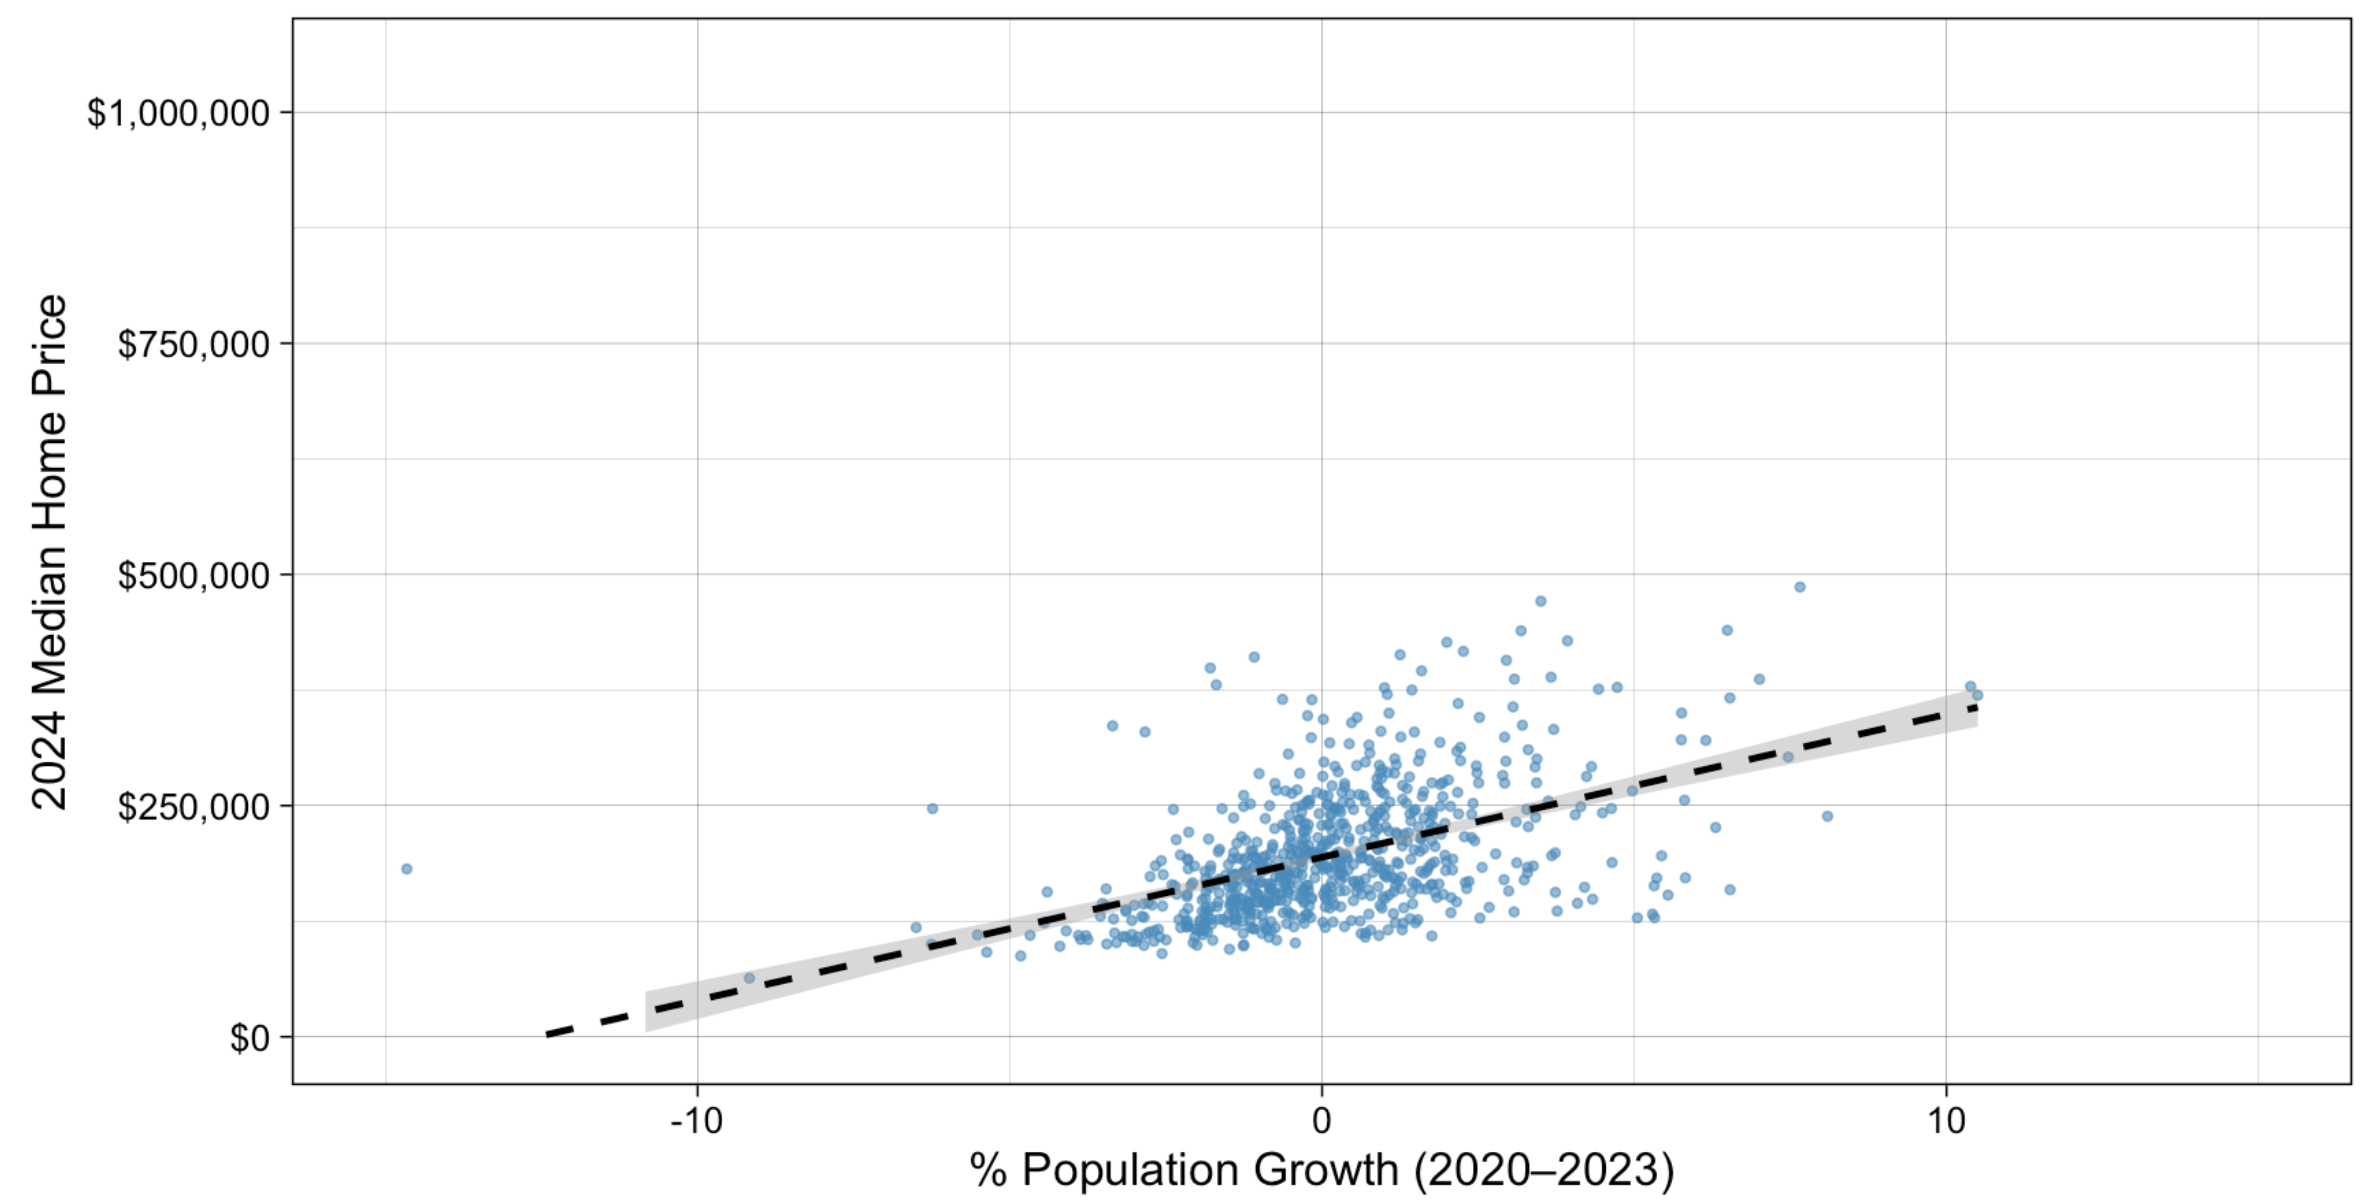
\includegraphics[width=0.88\textwidth]{fig13.png}
  \caption{\textbf{County Population Growth vs. Median Home Prices (2020–2023)}\\
  \textit{Midwestern U.S. Counties}}
  \label{fig:figure13}
  \vspace{1ex}
  {\footnotesize\textit{Data Source: National Association of Realtors, United States Census Bureau}}
\end{figure}
 
\textbf{Figure~\ref{fig:figure14}} takes the same approach as \textbf{Figure~\ref{fig:figure13}} but instead visualizes variation within the Southeastern region. Figure~14 reveals much larger dispersion in the results, with both population growth and housing prices being spread wider across Southeastern counties. There are several outliers in the data, as several counties have a population growth rate over $10\%$, with some median home prices exceeding \$900{,}000. Because of this, the Southeast can be seen to have a much more dynamic and diverse housing landscape, which can be caused by several factors. One major factor that can be seen is increases in population as people move into the Southeast, notably in areas like Florida, Georgia, North Carolina, and Tennessee. This rapid growth within parts of the Southeast causes inflation within the housing market, especially in heavily urban areas or hotspots. Regional inequality is more pronounced than in the Midwest, as affordable counties are spread throughout the region and surround higher-income areas.

%%%%% FIGURES 13, 14, 15
\begin{figure}[H]
  \centering
  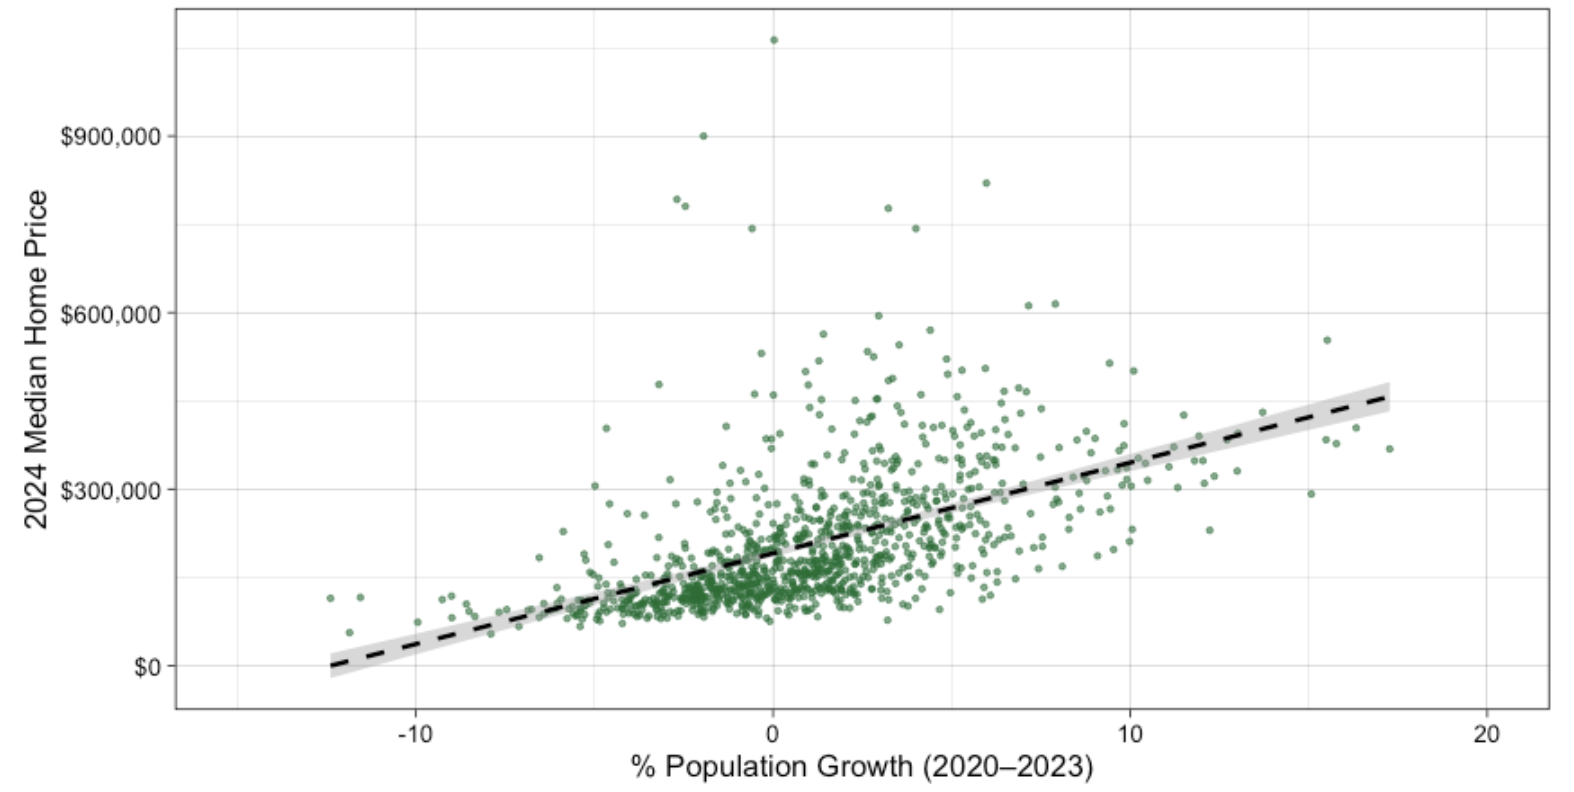
\includegraphics[width=0.88\textwidth]{fig14.png}
  \caption{\textbf{County Population Growth vs. Median Home Prices (2020–2023)}\\
  \textit{Southeastern U.S. Counties}}
  \label{fig:figure14}
  \vspace{1ex}
  {\footnotesize\textit{Data Source: National Association of Realtors, United States Census Bureau}}
\end{figure}
 
To directly compare the two regions, \textbf{Figure~\ref{fig:figure15}} overlays both regions onto one graph to explore the similarities and disparities between the two regions. Although both regions show a general positive correlation between population growth from 2020 to 2023 and median housing costs from 2024, the Southeast shows greater disparity and variability with its data. Midwestern counties dominate the lower left quadrant of Figure 15, which encourages lower growth, but lower prices and a softer entry point into the real estate market.

\begin{figure}[H]
  \centering
  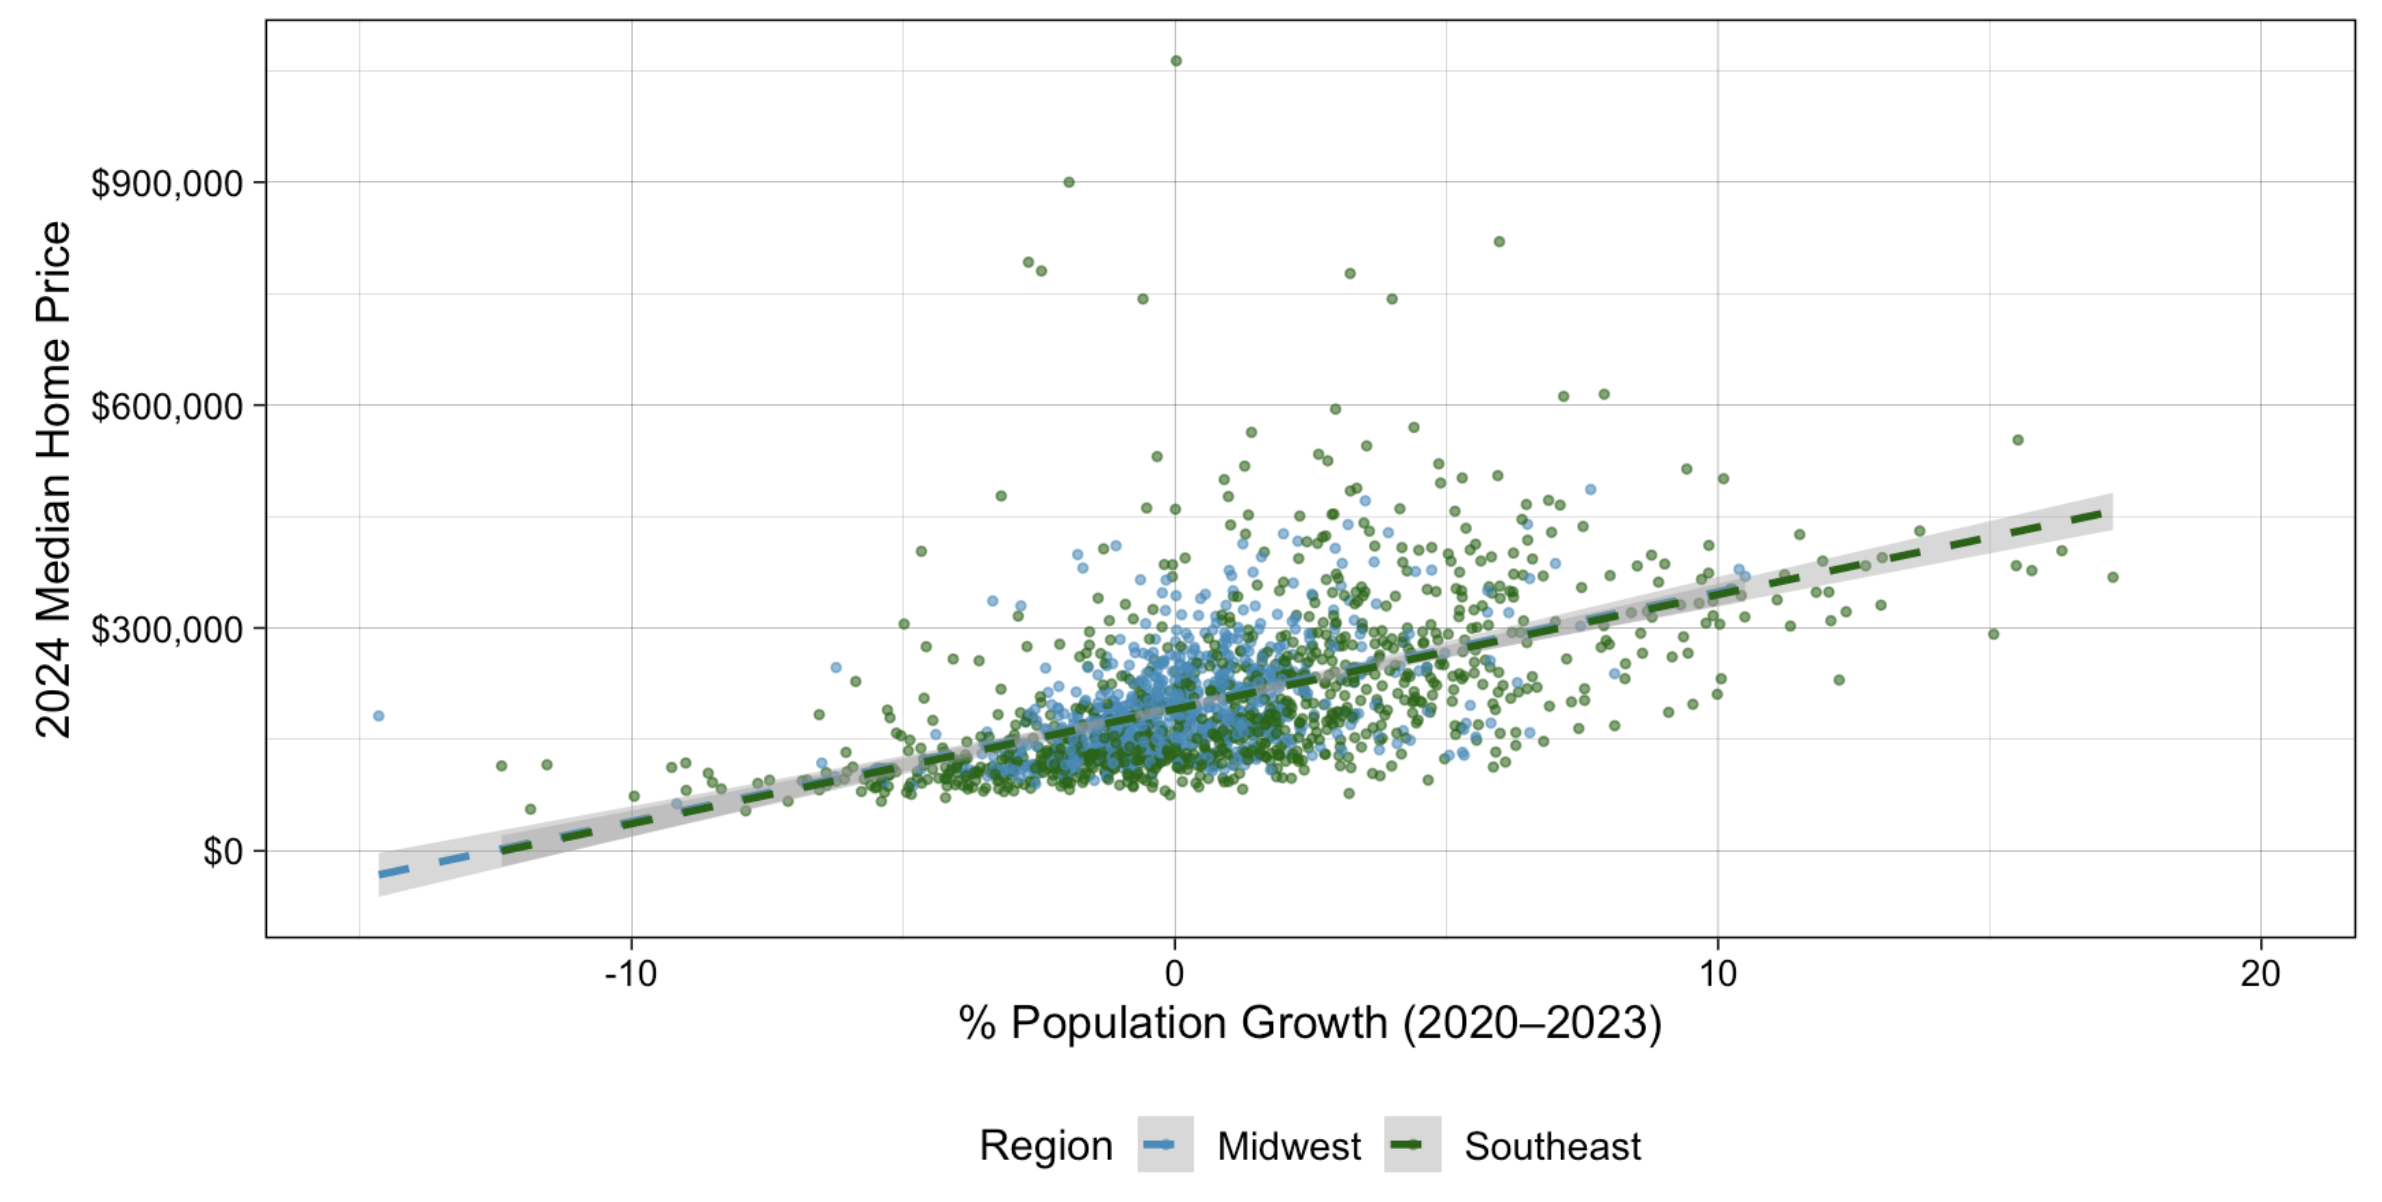
\includegraphics[width=0.88\textwidth]{fig15.png}
  \caption{\textbf{County Population Growth vs. Median Home Prices (2020–2023)}\\
  \textit{Comparison of Southeastern and Midwestern U.S. Counties}}
  \label{fig:figure15}
  \vspace{1ex}
  {\footnotesize\textit{Data Source: National Association of Realtors, United States Census Bureau}}
\end{figure}

 The overlap between the regions suggests that there are similarities between the regions, but the tails of the distribution tells the story that separates the two regions significantly. Several Midwestern counties showing high population density yet slower price growth, such as Columbus, OH or Indianapolis, IN, reflect how markets in the Midwest are more stable, and show a more consistent housing supply. This opposes the trends seen within the Southeast, as metros such as Nashville, TN and Charlotte, NC have more rapid price inflation, driven by stellar job growth and immigration. Outlier patterns in each region are often connected with metro areas in each region, where suburban spillover drives higher prices.

The comparative overlay also illustrates that the same amount of population growth over a time can influence two regions in dramatically different directions, which strengthens the argument that regional models are crucial for understanding the United States housing market as a whole. This graph also presents the issue that housing affordability issues are a growing phenomenon within the Southeastern region, and these issues are only trending upward. OpenAI’s models ChatGPT 4o and ChatGPT 03-mini-high were used within this research for grammar correction, formatting, and code troubleshooting \citep{openai_2025_chatgpt}.

\begin{comment}
\textcolor{red}{OpenAI’s models ChatGPT 4o and ChatGPT 03-mini-high were used within this research for grammar correction, formatting, and code troubleshooting \citep{openai_2025_chatgpt}.}
\end{comment}

%%%%%%%%%%%%%%%%%%%%%%%%%%%%%%%%%%%%%%%%%%

\section{Discussion}

The results of this research offer several different viewpoints on the complex interactions between population density and housing price dynamics within the Southeastern and Midwestern United States. These findings confirm the hypothesis that population growth and population density are significant drivers of housing demand and prices in both the Midwest and the Southeast. However, the hedonic model proved that while population density is important in some states, it cannot be relied on as the main determinant for predicting housing price across the United States, as there are significant variations among states within both regions. The comparison between these two regions is crucial for understanding the context behind the entire United States housing market, and these regions provide interesting and contrasting insights into this broader picture.
%\textcolor{red}{These findings confirm the hypothesis that population growth and population density are significant drivers of housing demand and prices in both the Midwest and the Southeast. However, the hedonic model proved that while population density is important in some states, it cannot be relied on as the main determinant for predicting housing price across the United States, as there are significant variations among states within both regions. The comparison between these two regions is crucial for understanding the context behind the entire United States housing market, and these regions provide interesting and contrasting insights into this broader picture.}

\subsection{Population Growth and Housing Price Divergence}

The Southeastern region’s rapid population growth fueled by immigration, economic conditions, and climate appeal corresponds with a highly volatile and accelerated housing market, which allows for unique investment opportunities despite a high barrier to entry.  This trend is substantiated by analyses through both the hedonic modeling as well as the ARIMA forecasts, which provide unique but encouraging results showing higher variability and drastic price increases in the Southeastern region. Several locations which embody these trends to a high degree are heavily urban counties within Florida, Tennessee, and North Carolina.

In contrast, the Midwest presents a more stable housing market, with less variability than that of the Southeastern market. Population trends within this region are either stagnant, or slightly increasing or decreasing, which correlates to more consistent and affordable home values. This trend allows for a softer barrier to entry within the Midwestern housing market, and its slower growth rate reduces the volatility present within the housing demand. This is reflected in both the historical HPI trends as well as trends within Zillow’s home value index data \citep{zillow_2024_housing}. These results found from both regions validate the necessity for regionally tailored housing prices, as the housing market varies significantly by region. The Southeast, for example, requires strategies to mitigate housing inflation to maintain some affordability, while the Midwest benefits from policies which may stimulate housing demand. This would allow for a softening of the housing inflation in the Southeast, while increasing housing demand and preventing market stagnation in the Midwest.

\subsection{Hedonic Insights: Mortgage Payments vs. Population Size}

The results from the hedonic model reveal that population size alone is not a strong enough predictor for housing costs, while monthly mortgage payments provide a much stronger prediction method. This explains that although more people in an area or county may increase housing demand, this alone is not a robust enough driver of price variation in housing costs. There are other factors that must be studied and considered when studying housing demand. This result challenges the simplistic narratives that assume rising home prices is solely caused by population growth and encourages the notion that housing affordability is shaped more heavily by market variables such as financing, as well as local economic conditions. However, population trends cannot be omitted, as they still follow very similar trends to housing prices over time.


\subsection{State Fixed Effects and Regional Disparities}

The state fixed effects component of the model also provides nuanced results. With Alabama as the base case state, states like Virginia or Missouri exhibit significantly lower housing prices relative to Alabama, while other state like Tennessee, North Carolina, and Florida exhibit mixed results while not being statistically significant. This is important to note as these trends can be seen within \textbf{Figure~\ref{fig:figure3}}, but more data is needed before gathering results from the choropleths. This variability is crucial to understand as even with a region growing as rapidly as the Southeast, there are still counties and even states which defy regional trends due to zoning laws, economic conditions, or geographical location. This implies that policymakers should avoid regional generalizations, as each county and state is unique in its structure and trends.
 
The ARIMA modeling demonstrated upward trends in both regions, although the Southeast is expected to have sharper increases in Housing Price Index and housing prices in the coming years. The Southeast’s ARIMA(2,2,0) model implies higher momentum and reliance on historical data, while the Midwest’s ARIMA(0,2,2) model shows steadier and stable growth within its housing market.


\subsection{Limitations}

While the models within this paper provide robust results, there are several limitations that must be addressed.
 
The first is that this study cannot claim causality, and the nature of this research is observational. Although fixed effects and time series controls reduce bias, there may still be unobserved factors which are not present in the models.
 
The next limitation is that county-level data provides strong resolution to these results and models but could obscure dynamics which are present at a smaller level, such as within a metropolitan area or around residential pockets in a city.
 
The third limitation that forecasting with time-series data is useful within this study but are limited by their reliance on past trends and historical data. This limitation is mitigated by the use of carefully constructed and outlined confidence intervals, providing proper context for each model and predictive forecast used.

\subsection{Conclusions}

This research contributes a regional comparative lens between these two crucial regions within the United States, an approach which is often missing in national-level research. By combining visual, statistical, and predictive techniques, this paper facilitates a widespread and multifaceted understanding of the intertwined dynamic between population dynamics and housing markets. These findings inform urban planners who may adapt zoning and infrastructure for increased growth within booming counties, policymakers who aim to preserve affordability within high-demand urban markets, real estate developers seeking to anticipate future market trends, and researchers who aim to refine econometric and spatial housing models with current and reliable data.

\subsection{Project Repository}
\noindent\url{https://github.com/christianmcintire/DACapstone}

%%%%%%%%%%%%%%%%%%%%%%%%%%%%%%%%%%%%%%%%%%


%%%%%%%%%%%%%%%%%%%%%%%%%%%%%%%%%%%%%%%%%%
% References
%%%%%%%%%%%%%%%%%%%%%%%%%%%%%%%%%%%%%%%%%%
\begin{adjustwidth}{-\extralength}{0cm}

\clearpage
\phantomsection
\addcontentsline{toc}{section}{References}
\section{References}

\begin{thebibliography}{99}

\bibitem{desilver2024}
DeSilver, D. (2024, October 25). \textit{A look at the state of affordable housing in the U.S.}. Pew Research Center. \url{https://www.pewresearch.org/short-reads/2024/10/25/a-look-at-the-state-of-affordable-housing-in-the-us/}

\bibitem{holly_2010_a}
Holly, S., Pesaran, M. H., & Yamagata, T. (2010). A spatio-temporal model of house prices in the USA. \textit{Journal of Econometrics, 158}(1), 66–82. \url{https://www.sciencedirect.com/science/article/pii/S0304407610000837} \href{https://doi.org/10.1016/j.jeconom.2010.03.040}{https://doi.org/10.1016/j.jeconom.2010.03.040}

\bibitem{suhaida_2011_housing}
Suhaida, M. S., Tawil, N. M., Hamzah, N., Che-Ani, A. I., Basri, H., & Yuzainee, M. Y. (2011). Housing affordability: A conceptual overview for house price index. \textit{Procedia Engineering, 20}, 346–353. \url{https://www.sciencedirect.com/science/article/pii/S1877705811029857} \href{https://doi.org/10.1016/j.proeng.2011.11.176}{https://doi.org/10.1016/j.proeng.2011.11.176}

\bibitem{souders_2016_the}
Souders, A., Renna, F., & Weinstein, A. (2016). \textit{The effect of population density on housing prices: A cross state analysis}. University of Akron. \url{https://www.uakron.edu/economics/academics/senior-projects/2016/Souders-A-SeniorProject2016.pdf}

\bibitem{sirmans_2005_the}
Sirmans, G. S., Macpherson, D. A., & Zietz, E. N. (2005). The composition of hedonic pricing models. \textit{Journal of Real Estate Literature, 13}(1), 3–43. \url{https://www.jstor.org/stable/44103506} \href{https://doi.org/10.2307/44103506}{https://doi.org/10.2307/44103506}

\bibitem{_2024_net}
United States Census Bureau. (2024). \textit{Net international migration drives highest U.S. population growth in decades}. \url{https://www.census.gov/newsroom/press-releases/2024/population-estimates-international-migration.html}

\bibitem[Johnson and Lichter(2019)]{johnson_2019_rural}
Johnson, K., \& Lichter, D. (2019). \textit{Rural Depopulation in a Rapidly Urbanizing America}. Issue Lab (Candid). \url{https://scholars.unh.edu/carsey/358/?utm_source=chatgpt.com} \doi{10.34051/p/2020.347}

\bibitem[eXp Realty(2024)]{a2024_how}
eXp Realty. (2024, July). \textit{How Has Population Growth Affected Home Prices?} eXp Life. \url{https://life.exprealty.com/analysis-population-growth-affected-home-prices/}

\bibitem[Gupta et al.(2021)]{gupta_2021_flattening}
Gupta, A., Mittal, V., Peeters, J., \& Van Nieuwerburgh, S. (2021). Flattening the curve: Pandemic-induced revaluation of urban real estate. \textit{Journal of Financial Economics, 146}(2). \doi{10.1016/j.jfineco.2021.10.008}

\bibitem[National Association of Realtors(2024)]{_2024_county}
National Association of Realtors. (2024). \textit{County Median Home Prices and Monthly Mortgage Payment, Q3 2024}. \url{https://www.nar.realtor/research-and-statistics/housing-statistics/county-median-home-prices-and-monthly-mortgage-payment}

\bibitem[Federal Reserve Bank of St. Louis(2024a)]{a2024_resident_se}
Federal Reserve Bank of St. Louis. (2024, December). \textit{Resident Population in the Southeast BEA Region}. \url{https://fred.stlouisfed.org/series/BEASEPOP}

\bibitem[Federal Reserve Bank of St. Louis(2024b)]{a2024_resident_mw}
Federal Reserve Bank of St. Louis. (2024, December). \textit{Resident Population in the Midwest Census Region}. \url{https://fred.stlouisfed.org/series/CMWRPOP}

\bibitem[United States Census Bureau(2023)]{_2023_county}
United States Census Bureau. (2023). \textit{County Population Totals and Components of Change: 2020--2023}. \url{https://www.census.gov/data/tables/time-series/demo/popest/2020s-counties-total.html}

\bibitem[United States Census Bureau(2024a)]{_2024_state}
United States Census Bureau. (2024). \textit{State Population Totals and Components of Change: 2020--2024}. \url{https://www.census.gov/data/tables/time-series/demo/popest/2020s-state-total.html}

\bibitem[Zillow(2024)]{zillow_2024_housing}
Zillow. (2024). \textit{Housing Data - Zillow Research}. \url{https://www.zillow.com/research/data/}

\bibitem[Federal Reserve Bank of St. Louis(2024)]{a2024_hpi}
Federal Reserve Bank of St. Louis. (2024). \textit{HPI, State - Economic Data Series}. \url{https://fred.stlouisfed.org/tags/series?t=hpi%3Bstate}

\bibitem[Cooper \& Coetzee(2020)]{cooper_2020_on}
Cooper, A. K., \& Coetzee, S. (2020). On the ethics of using publicly-available data. \textit{Lecture Notes in Computer Science}, \textit{12067}, 159--171. \url{https://doi.org/10.1007/978-3-030-45002-1_14}

\bibitem[Chau \& Chin(2003)]{chau_2003_a}
Chau, K. W., \& Chin, T. L. (2003). A critical review of literature on the hedonic price model. \textit{International Journal for Housing Science and Its Applications}, \textit{27}, 145--165. \url{https://www.researchgate.net/publication/255726402_A_Critical_Review_of_Literature_on_the_Hedonic_Price_Model}

\bibitem[Herath \& Maier(2010)]{herath_2010_the}
Herath, S., \& Maier, G. (2010). The hedonic price method in real estate and housing market research: A review of the literature. \url{https://research.wu.ac.at/ws/portalfiles/portal/30983294/sre-disc-2010_03.pdf} \url{https://doi.org/10.57938/e55da0fe-d130-415d-9a5d-7bbc07c329a1}

\bibitem[He(2023)]{he_2023_influence}
He, Q. (2023). Influence factor analysis and forecast of US house prices based on linear regression and time series. \textit{Advances in Economics, Management and Political Sciences}, \textit{64}, 251--262. \url{https://doi.org/10.54254/2754-1169/64/20231543}

\bibitem[Brinkmann(2009)]{brinkmann_2009_putting}
Brinkmann, J. (2009). Putting ethics on the agenda for real estate agents. \textit{Journal of Business Ethics}, \textit{88}, 65--82. \url{https://doi.org/10.1007/s10551-009-0099-8}

\bibitem[Ekeland et al.(2004)]{ekeland_2004_identification}
Ekeland, I., Heckman, J. J., \& Nesheim, L. (2004). Identification and estimation of hedonic models. \textit{Journal of Political Economy}, \textit{112}(S1), S60--S109. \url{https://doi.org/10.1086/379947}

\bibitem[Liu(2024)]{liu_2024_navigating}
Liu, J. (2024). Navigating the financial landscape: The power and limitations of the ARIMA model. \textit{Highlights in Science, Engineering and Technology}, \textit{88}, 747--752. \url{https://drpress.org/ojs/index.php/HSET/article/view/19082} \url{https://doi.org/10.54097/9zf6kd91}

\bibitem[Torres-Reyna(2010)]{torresreyna_2010_getting}
Torres-Reyna, O. (2010). \textit{Getting started in fixed/random effects models using R (ver. 0.1-Draft)}. \url{https://www.princeton.edu/~otorres/Panel101R.pdf}

\bibitem[Aladwan and Ahamad(2019)]{aladwan_2019_hedonic}
Aladwan, Z., \& Ahamad, M. S. S. (2019). Hedonic pricing model for real property valuation via GIS – A review. \textit{Civil and Environmental Engineering Reports}, \textit{29}(3), 34–47. \url{https://doi.org/10.2478/ceer-2019-0022}

\bibitem[R Core Team(2024)]{rcoreteam_2024_r}
R Core Team. (2024). \textit{R: A language and environment for statistical computing}. R Foundation for Statistical Computing. \url{https://www.r-project.org/}

\bibitem[Biernacka-Lievestro and Fall(2023)]{biernackalievestro_2023_southern}
Biernacka-Lievestro, J., \& Fall, A. (2023, May). Southern states gain residents the fastest. \textit{pew.org}. \url{https://www.pewtrusts.org/en/research-and-analysis/articles/2023/05/17/southern-states-gain-residents-the-fastest}

\bibitem[Maynard and Fall(2021)]{maynard_2021_population}
Maynard, M., \& Fall, A. (2021, July). Population growth sputters in Midwestern, Eastern states. \textit{pew.org}. \url{https://www.pewtrusts.org/en/research-and-analysis/articles/2021/07/27/population-growth-sputters-in-midwestern-eastern-states}

\bibitem[United States Census Bureau(2024)]{unitedstatescensusbureau_2024_tigerline}
United States Census Bureau. (2024, January). \textit{TIGER/Line shapefiles}. The United States Census Bureau. \url{https://www.census.gov/geographies/mapping-files/time-series/geo/tiger-line-file.html}

\bibitem[Holtz(n.d.)]{holtz_choropleth}
Holtz, Y. (n.d.). Choropleth map with R and ggplot2. \textit{www.r-graph-gallery.com}. \url{https://r-graph-gallery.com/327-chloropleth-map-from-geojson-with-ggplot2.html}

\bibitem[GeeksforGeeks(2021)]{geeksforgeeks_2021_control}
GeeksforGeeks. (2021, May). Control size of ggplot2 legend items in R. \textit{GeeksforGeeks}. Retrieved March 15, 2025, from \url{https://www.geeksforgeeks.org/control-size-of-ggplot2-legend-items-in-r/}

\bibitem[OpenAI(2025)]{openai_2025_chatgpt}
OpenAI. (2025). \textit{ChatGPT}. ChatGPT. \url{https://chatgpt.com/}


\end{thebibliography}


%%%%%%%%%%%%%%%%%%%%%%%%%%%%%%%%%%%%%%%%%%

\clearpage
\phantomsection
\addcontentsline{toc}{section}{References}
\section{Appendix}

\subsection*{United States Census Bureau Dataset Cleaning}


\begin{itemize}
  \setlength\itemsep{0pt}
  \setlength\parskip{0pt}
  \setlength\parsep{0pt}
  \item The data is cleaned in Excel prior to analysis in R. The cleaned dataset is saved in Sheet2, named ``cleaned\_data''.
  \item Column headers are renamed for clarity: \texttt{County}, \texttt{estimate\_april\_1\_2020}, \texttt{2020\_pop}, \texttt{2021\_pop}, \texttt{2022\_pop}, and \texttt{2023\_pop}.
  \item The dataset is filtered in RStudio to include only counties from selected Southeastern and Midwestern states.
\end{itemize}

These cleaning and filtering steps allow for seamless merging with the county-level home price data and facilitate accurate visualization and modeling.

\begin{comment}
{\color{red}
\begin{itemize}
  \setlength\itemsep{0pt}
  \setlength\parskip{0pt}
  \setlength\parsep{0pt}
  \item The data is cleaned in Excel prior to analysis in R. The cleaned dataset is saved in Sheet2, named ``cleaned\_data''.
  \item Column headers are renamed for clarity: \texttt{County}, \texttt{estimate\_april\_1\_2020}, \texttt{2020\_pop}, \texttt{2021\_pop}, \texttt{2022\_pop}, and \texttt{2023\_pop}.
  \item The dataset is filtered in RStudio to include only counties from selected Southeastern and Midwestern states.
\end{itemize}
}

{\color{red}{These cleaning and filtering steps allow for seamless merging with the county-level home price data and facilitate accurate visualization and modeling.}
\end{comment}



\end{adjustwidth}
\end{document}
%%%%%%%%%%%%%%%%%%%%%%%%%%%%%%%%%%%%%%%%%%
